%%%%%%%%%%%%%%%%%%%%%%%%%%%%%%%%%%%%%%%%%%%%%%%%%%%%%%%%%%%%%%%%%%%%%%%%%%%%%%%%
%2345678901234567890123456789012345678901234567890123456789012345678901234567890
%        1         2         3         4         5         6         7         8
%\documentclass[letterpaper, 10 pt, conference]{ieeeconf}  % Comment this line out
                                                           % if you need a4paper
\documentclass[a4paper, 10pt, conference]{ieeeconf}        % Use this line for a4
                                                           % paper

\IEEEoverridecommandlockouts                               % This command is only
                                                           % needed if you want to
                                                           % use the \thanks command
\overrideIEEEmargins
% See the \addtolength command later in the file to balance the column lengths
% on the last page of the document
% packages
\usepackage{epsf, epstopdf,	graphicx, xcolor, 
			latexsym,
			anysize, % for margins left, right top bottom
			setspace, cite,	moreverb,
			fancyhdr, %does the headers on the pages - keep in
			algorithm, url,
			%hyperref,
			algorithmic, subfigure, 
			booktabs,
			multirow, % table
			wrapfig, tabularx,  % table tool
			colortbl,  % color in table
			multirow,  % table package
			rotating, empheq, bbding,    % for table details
			pifont,     % for table details
			fmtcount			
			}

% The following packages can be found on http:\\www.ctan.org
%\usepackage{graphics} % for pdf, bitmapped graphics files
%\usepackage{epsfig} % for postscript graphics files
%\usepackage{mathptmx} % assumes new font selection scheme installed
%\usepackage{times} % assumes new font selection scheme installed
\usepackage{amsmath} % assumes amsmath package installed
\usepackage{amssymb}  % assumes amsmath package installed
\usepackage{authblk}

%%%%% my add-ons %%%%%
\newcommand{\vect}[1]{\boldsymbol{#1}}
\newcommand{\T}{\texttt}

\title{\LARGE \bf
Underwater Vehicle Localisation using Extended Kalman Filter
}
%\author{Miroslav Radojevi\'{c}\thanks{M. Radojevi\'{c} is a student in ViBot programme, {\tt \small miroslav.radojevic@gmail.com}} and Yvan Petillot\thanks{Y. Petillot is with the Oceans Systems Laboratory, Heriot-Watt University, Edinburgh, UK}}
\author[1]{Miroslav Radojevi\'{c}}
\author[2]{Yvan Petillot}
\affil[1]{Erasmus Mundus Master in Computer Vision and Robotics (ViBot) student}
\affil[2]{Ocean Systems Laboratory, Heriot-Watt University, Edinburgh, UK}
\begin{document}

\maketitle
\thispagestyle{empty}
\pagestyle{empty}

\let\oldthefootnote\thefootnote
\renewcommand{\thefootnote}{\fnsymbol{footnote}}
\footnotetext[1]{To whom correspondence should be addressed. Email: \url{miroslav.radojevic@gmail.com}}
\let\thefootnote\oldthefootnote


\renewcommand{\topfraction}{0.85}
\renewcommand{\textfraction}{0.1}
\renewcommand{\floatpagefraction}{0.75}
%%%%%%%%%%%%%%%%%%%%%%%%%%%%%%%%%%%%%%%%%%%%%%%%%%%%%%%%%%%%%%%%%%%%%%%%%%%%%%%%
\begin{abstract}
In order to accomplish various missions, autonomous underwater vehicles (AUVs) need to be capable of estimating their position within the environment. This is a prerequisite of a successful mission since further tasks strongly rely on navigation information. This paper presents the application of an algorithm that would accomplish the localisation of the Ocean Systems Lab's Nessie underwater vehicle using measurements from a number of sensors mounted on it. Well known Extended Kalman Filter (EKF) algorithm approach was suggested as a solution for robot self-localisation. Additional practical issue that was addressed in the work is the choice of heading sensor and quality of the obtained heading as an important ingredient of the navigation. Implementation of the Unscented Kalman Filter (UKF) was investigated as potential improvement in working with nonlinearities. Finally, the absolute position observations tend to be quite noisy but very important measurements for navigation. EKF was demonstrated as a tool for sensor fusion and simultaneous filtering of the position measurements. Experiments with recorded real-time sensor data and real missions have been carried out. Their results have been presented as a part of navigation performance test and analysis. 
\end{abstract}
%%%%%%%%%%%%%%%%%%%%%%%%%%%%%%%%%%%%%%%%%%%%%%%%%%%%%%%%%%%%%%%%%%%%%%%%%%%%%%%%
\section{INTRODUCTION} \label{sec:intro}
This paper is reporting the application of EKF for localisation of the above mentioned Nessie AUV in an unstructured environment. The concept of sensor fusion was explained. The main contribution is the implementation of an EKF estimator adopted to work on a real underwater vehicle with real-time signals received from sensors. Five degrees of freedom (5DOF) model of the vehicle dynamics was introduced to take the role of the prediction. Work examines the problem from the perspective of engineering a successful AUV navigation in general. The issue of accurate heading and the outliers in absolute position measurement was analysed. Unscented Kalman Filter (UKF) \cite{julier96} was implemented as an attempt to improve the performance and compensate for the shortcomings of the EKF.  

Paper is organised as follows: section \S~\ref{sec:cap} gives an overview of AUV's navigation capabilities. Section \S~\ref{sec:ekf} introduces the theory of EKF. Section \S~\ref{sec:sensors} briefly presents each of the measurement devices. Implementation of the localisation module was detailed in section \S~\ref{sec:implementation}. Finally, results are shown in section \S~\ref{sec:results} ending with conclusions and future work in section \S~\ref{sec:concl}.
%%%%%%%%%%%%%%%%%%%%%%%%%%%%%%%%%%%%%%%%%%%%%%%%%%%%%%%%%%%%%%%%%%%%%%%%%%%%%%%%
\section{NAVIGATION CAPABILITIES OF AUVs} \label{sec:cap}
\begin{figure}%[htp]
  \begin{center}
    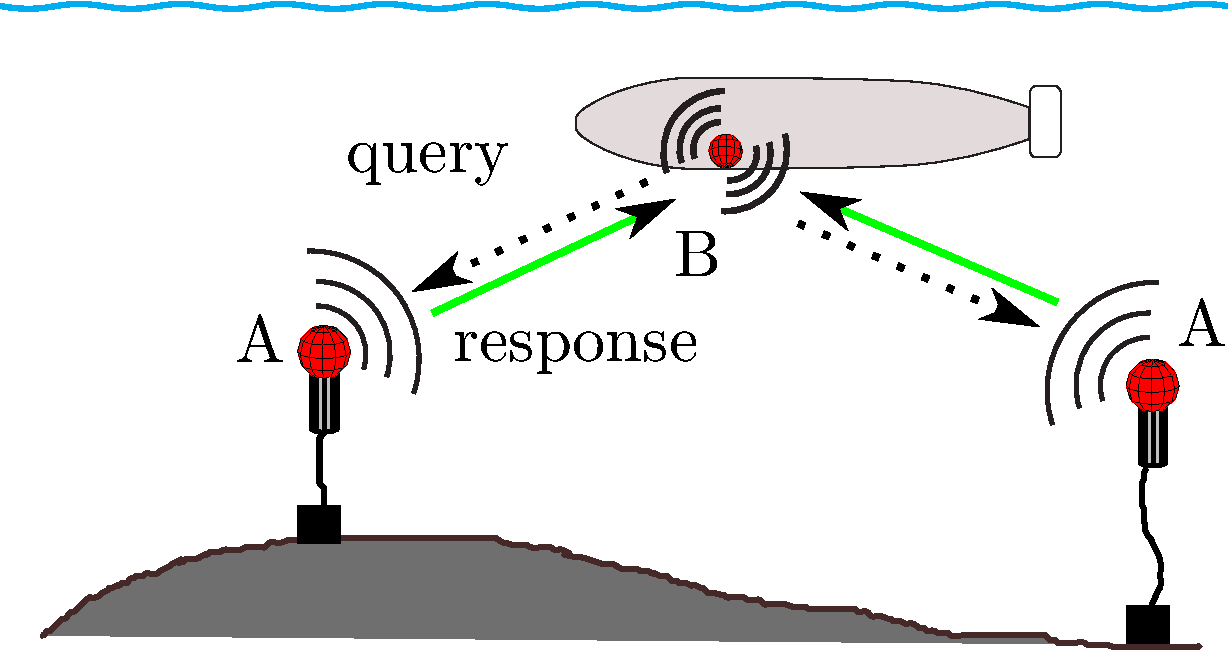
\includegraphics[width=0.4\textwidth]{standard-lbl.pdf}
  \end{center}
  \caption{Standard LBL: A - transponder, B - transducer. Acoustic waves are exchanged between A and B. Detected ``time-of-flight'' is used to estimate the distance between, hence the position in the network of transponders.}
  \vspace{-10pt}
  \label{fig:lbl}
\end{figure}
Primary navigation system in most of the applications, including underwater navigation, is Inertial Navigation System (INS) \cite{lawrence98}. Motion and rotation information obtained this way are processed in order to provide an estimate of objects location with respect to the initial reference. Since such system accumulates noisy data, it introduces the drift errors that need to be occasionally corrected inside the navigation algorithm. Various ways of correcting those errors were developed. Common ``correction tool'' is the incorporation of an absolute position measurement in form of GPS (\S~\ref{sec:sensors}) or acoustic acoustic based LBL (\S~\ref{sec:sensors}) available underwater (Figure ~\ref{fig:lbl}). Absolute position is inferred from the acoustic feedback of transponders so that the vehicle is capable of locating itself with respect to transponder network.
Carrying out underwater vehicle localisation implies introducing concepts such as \textit{vehicle state} within a navigation strategy framework. Vehicle navigation state describes its position within the environment. Vehicle state is a vector that contains variables relevant for localising the vehicle. In this work, state vector is treated as stochastic - consisted of random variables with Gaussian distribution. As it is the case with random variables, we can say that certain state has an expected value, and that such ``randomness'' can be expressed with the distribution formula, resulting in descriptor values such as mean and standard deviation that fully describe the distribution in particular case of Gaussian. Most notable stochastic state estimator is Kalman Filter (KF). KF works through iterations by employing the process model for making the \textit{state prediction} and the observations for doing the \textit{state correction} \cite{negenborn03}. Real world consists of various nonlinear systems. Practical situations often demand the usage of approximations that eventually lead to linearisation. EKF is a nonlinear version of KF which linearises about the current mean and covariance - hence uses analytic approximations. UKF, on the other hand, is based on sampling \cite{julier96}. Both treat random variable as Gaussian.
%%%%%%%%%%%%%%%%%%%%%%%%%%%%%%%%%%%%%%%%%%%%%%%%%%%%%%%%%%%%%%%%%%%%%%%%%%%%%%%%
\chapter{Kalman filtering} \label{chap:kalman}

\section{Linear filtering}
Idea is that the system can be described with set of states that evolve in time. There can be various number of states and all of them are grouped together in the state vector. Navigation system could, for instance, group together position coordinates and orientation angles in the state vector. If the system is considered as discrete, transition from one discrete value of the state vector to the next one, is described with the function $f$ called process model, equation ~\ref{eq:state-transition}, where the current state, $x(k+1)$, is calculated using the process model with prevoius state ($x(k)$), current input ($u(k+1)$) and process noise ($v(k+1)$) as arguments. In other words, model mathematically describes how the state changes for a given input. System formula ~\ref{eq:state-transition} is used as first stage of filtering.

\begin{equation}
\vect{x}(k+1) = \vect{f}[\vect{x}(k), \vect{u}(k+1), \vect{v}(k+1), k+1]
\label{eq:state-transition}
\end{equation}

Thus, our system is not entirely an unknown black box once a linear Kalman Filter(KF) is attached to it. A hint about its dynamics is known in form of process model. The only information available once the filtering starts, are its control inputs ($u$) and a set of observations ($z$). equation ~\ref{eq:state-observation} associates observations with the state. Similarly as shown in ~\ref{eq:state-transition}, $x$ and $u$ present the state, while $w$ represents the additive measurment noise and function $h$ observation model \cite{julier96}.
 
\begin{equation}
\vect{z}(k+1) = \vect{h}[\vect{x}(k+1), \vect{u}(k+1), k+1] + \vect{w}(k+1)
\label{eq:state-observation}
\end{equation} 
 
Assumptions that KF uses:
\begin{itemize}
\item distribution of a random variable is assumed to be Gaussian, therefore mean and variance can fully describe it
\item linear transform of a Gaussian distribution gives another Gaussian distribution 
\end{itemize}
In spirit of that, noise vectors and thus linearly derivated state and observation vectors are Gaussian. Another assumption is that noise vectors $v$, $w$ have zero mean values and that their elemets are not correlated, which was stated in equations ~\ref{eq:noise}.

\begin{equation}
\begin{split}
E \left[ \vect{v}(i) \vect{v}^{T}(j) \right]  = \delta_{ij} \vect{Q}(i) \\
E \left[ \vect{w}(i) \vect{w}^{T}(j) \right]  = \delta_{ij} \vect{R}(i) \\
E \left[ \vect{v}(i) \vect{w}^{T}(j) \right]  = \vect{0}, \forall i,j
\end{split} 
\label{eq:noise}
\end{equation}

Kalman filter is a well known algorithm, covered in various literature \cite{grewal01}, \cite{ristic04}. Discrete Kalman Filter is an optimal unbiased minimum mean squared error estimator. It is a calculation process that works recursively, passing iterations as shown in diagram ~\ref{fig:diagram-kalman}. One iteration uses equation ~\ref{eq:state-transition}, next one uses equation ~\ref{eq:state-observation} and the recursion continues with having new prediction and correction of that observation each cycle.   

\begin{figure}[h!]
  \centering
    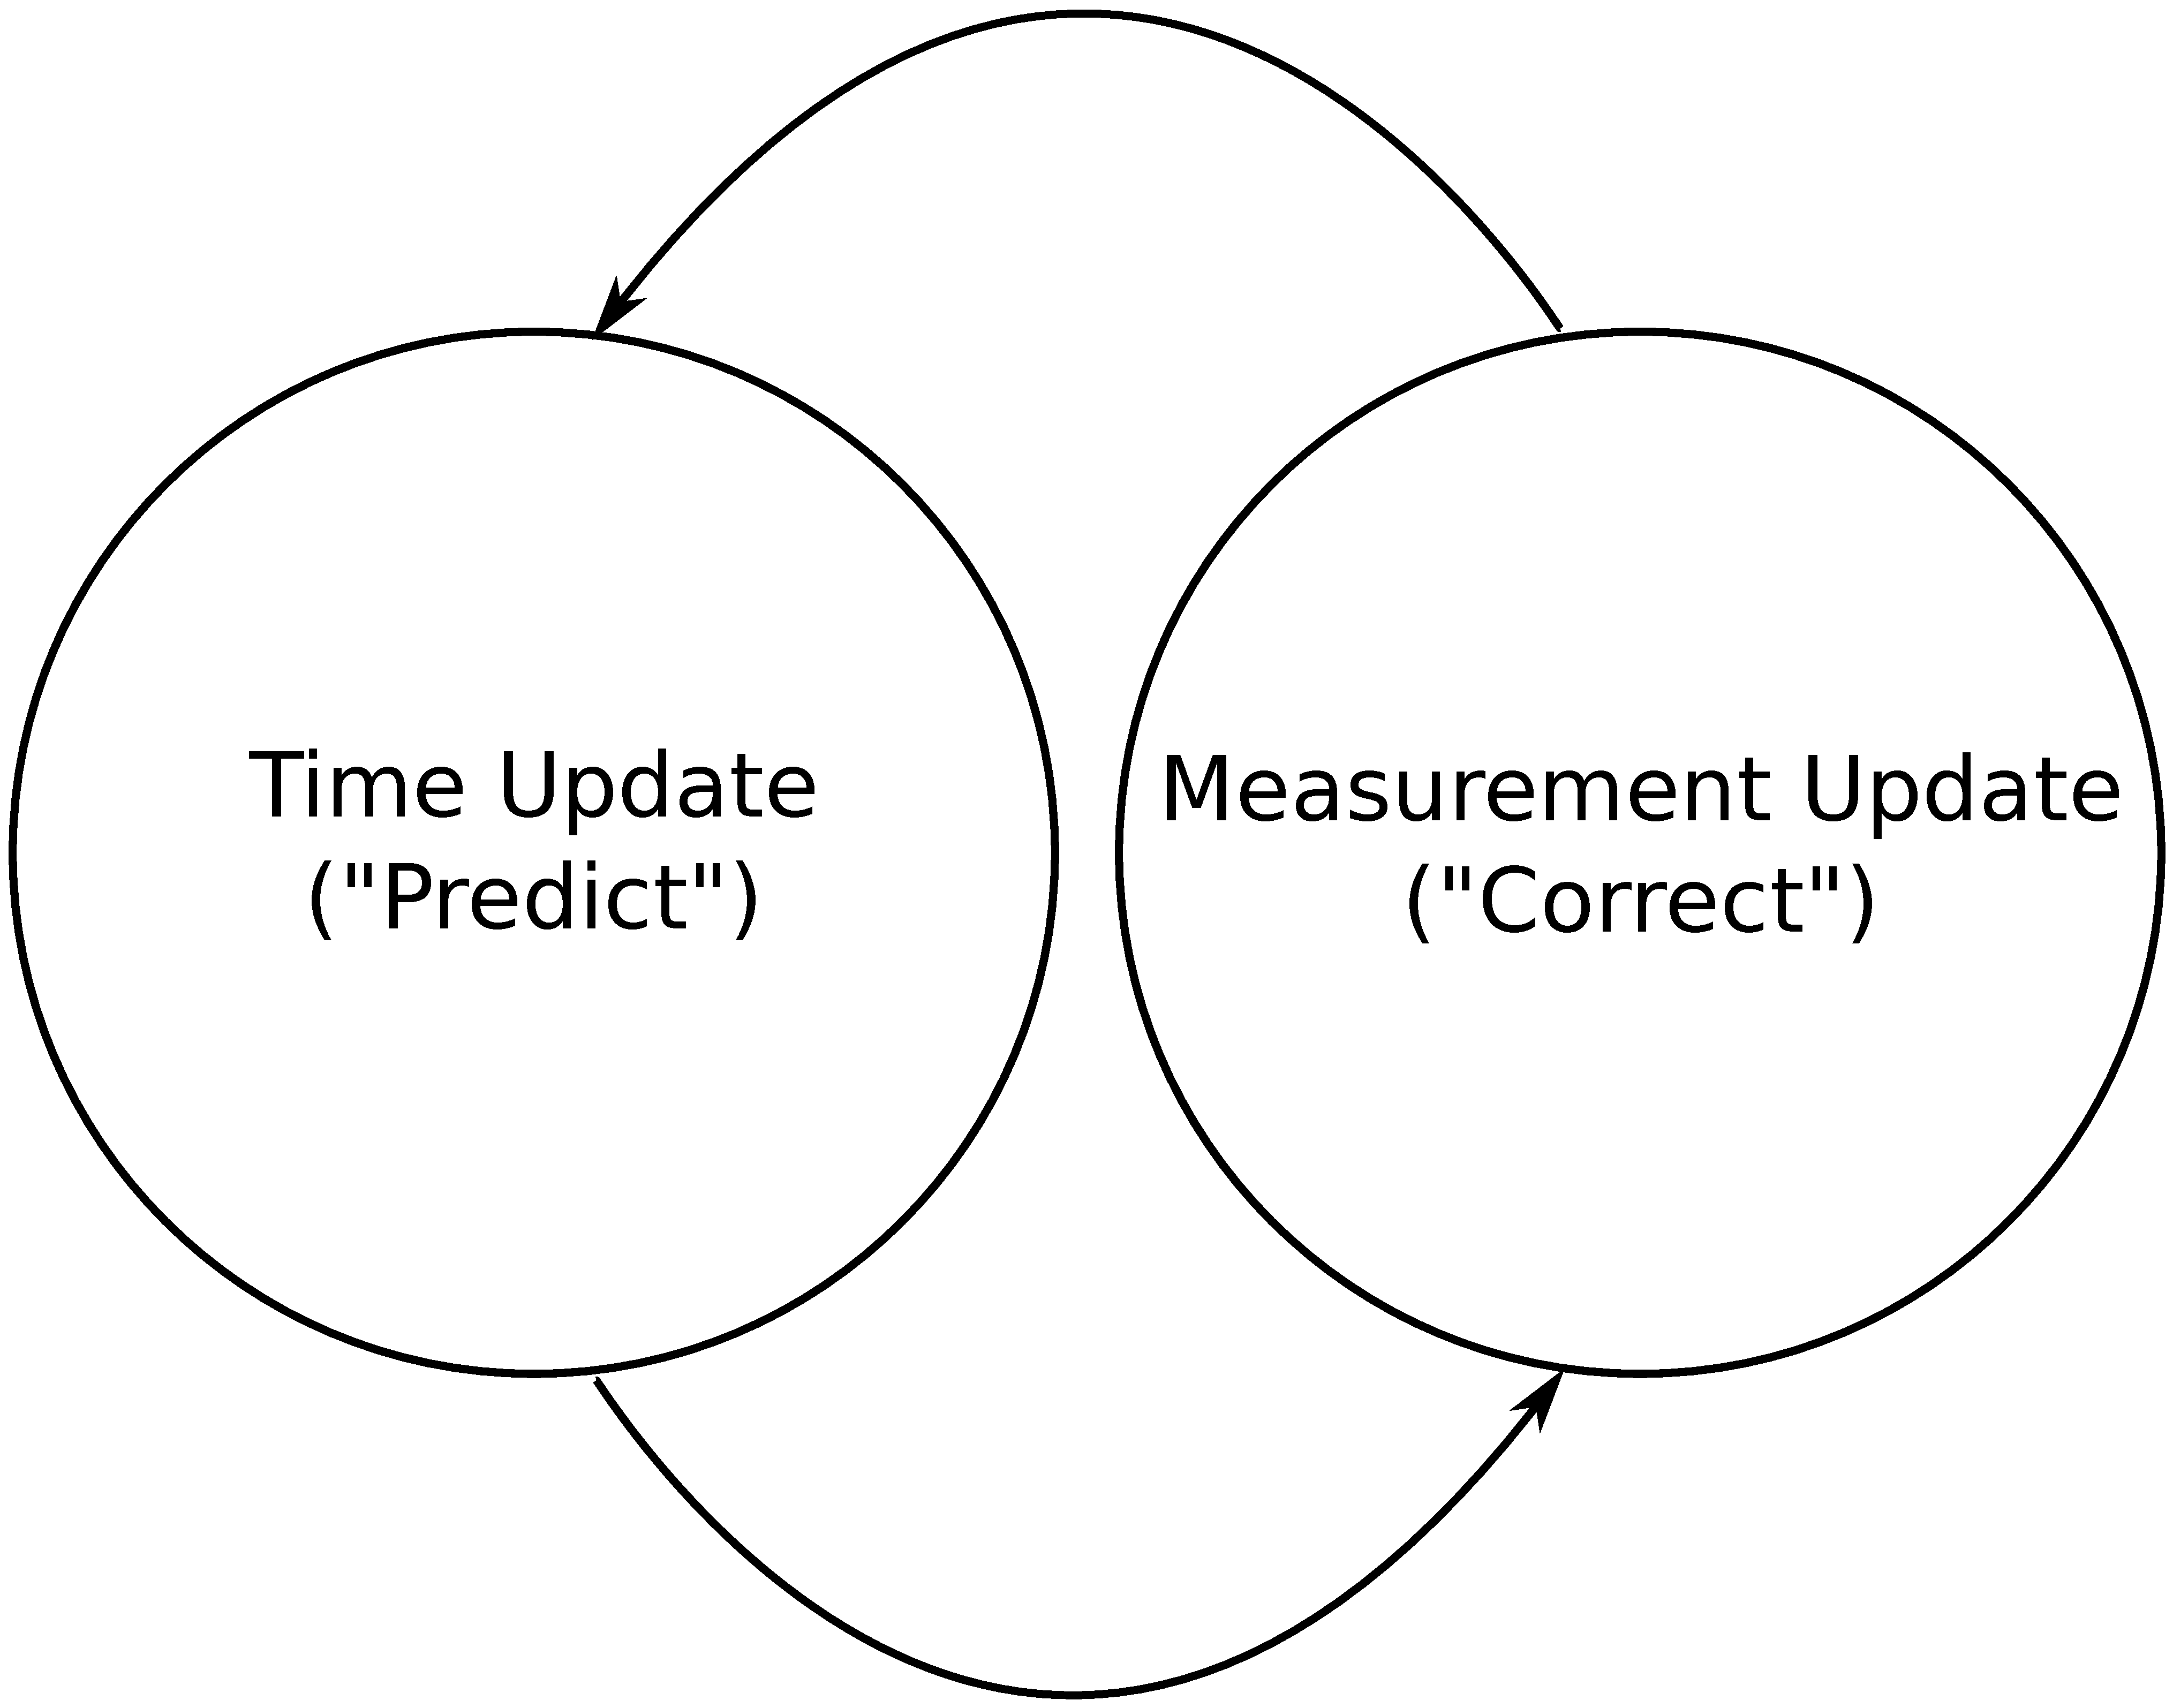
\includegraphics[width=0.5\linewidth]{kalman/fig/diagram-kalman.eps}
  \caption{Filtering process.}
\label{fig:diagram-kalman}
\end{figure}

One of its particularly useful features is the ability to combine together sensor measurements in mathematical form such that the solution is best possible estimate of the mean and the variance. 

Kalman filter uses three basic stages: prediction measurement and update. This would mean that the mean and the variance of the state are measureable. Prediction in case of moving vehicle is calculated based on previous vehicle location and dead reckoning.

Kalman gain determines the relationship between the importance of each previous estimation () and the current measurement (). Essentially - it expresses how much we trust in the measurement with respect to what we prediceted. According to the formula (), it is determined by matrices $Q$ and $R$ which represent process noise covariance and the measurement noise covariance (uncertainty), respectively. It takes values between 0 and 1 with 0 meaning that we use estimation only and give no importance to the measurement, and 1 that we consider direct measurement as the only important one.   

\section{Extended Kalman Filter (EKF)}

Real world models are rarely linear. The motiv for developing the Extended Kalman Filter is the adaptation of the linear Kalman Filter to dealing with nonlinear problems. However, it is possible that EKF significantly declines the performance quality \cite{julier96}. When making a prediction of state, observation or uncertainty of any of those for nonlinear systems, linearization can introduce errors. One example of such case is given in \cite{julier96}. The object follows the circular path. In such quite common case, the reason for failing in prediction is in linear approximations that EKF, by nature, uses when predicting the next state and its characteristics.

\section{Unscented Kalman Filter (UKF)}
Calculation-wise, the whole procedure is better than linearisation algorithm since there is no need for calculating the Jacobian, number of computations stays the same and it is easier to improvise with the algorithm by constraining or changing the samples \cite{julier96}.
\begin{algorithm}
\caption{UKF algorithm}
\label{alg:ukf}                   
%%%\begin{algorithmic}
%%%\INPUT state vector
%%%\OUTPUT feature vector \textit{fea}
%%%\FOR{$dist=0$ to $10$}
%%%\FORALL{$dir$ in \{0, 45, 90, 135\}}
%%%\STATE $glcm \leftarrow compute\ co-occurrence\ matrix\ for\ each\ pair\ of\ dist-dir$
%%%\STATE $normglcm \leftarrow normalize\ GLCM\ with\ the\ number\ of\ occurences$
%%%\STATE $harfea \leftarrow compute\ Haralick\ features$ \COMMENT{as in Appendix A}
%%%\STATE $fea \leftarrow [fea\ harfea]$ \COMMENT{store in feature vector}
%%%\ENDFOR
%%%\ENDFOR
%%%\end{algorithmic}
\end{algorithm}
%%%%%%%%%%%%%%%%%%%%%%%%%%%%%%%%%%%%%%%%%%%%%%%%%%%%%%%%%%%%%%%%%%%%%%%%%%%%%%%%
\section{SENSORS} \label{sec:sensors}
Underwater positioning can utilise different types of sensors combined together in one system. The role of the sensors is to measure absolute position, velocities and heading/orientation. Sensor outputs measure with reference either in \textit{body frame} (Figure ~\ref{fig:auv-axes}), the one fixed to the object or in \textit{global frame} (Figure ~\ref{fig:auv-positioning}). Basic navigation sensor set for a high-end AUV usually consists of:% depth sensor, magnetic compass, GPS device, LBL acoustic device, Doppler Velocity Log (DVL) and fibre-optic gyroscope (FOG).

\T{Pressure (depth) sensor} is standard piece of the equipment for an AUV. Measuring the pressure enables the correlation of the value of pressure with the value of depth. Device can frequently ascertain the absolute depth with good precision, within the range of centimetres. 

\T{Magnetic compass} provides 3D vector of local magnetic field. It's main role is orientation measurement, particularly heading (yaw). Magnetic compass points at magnetic north. North direction as it appears on maps points to the geographic north (``true north''). That is the direction towards the rotation axis of the Earth. Magnetic declination is an angle between magnetic north (measured by compass) direction and the true north direction (the one that maps refer to). Depending on location where the compass is used, magnetic declination can vary, hence, calibration is necessary. In addition, different magnetic effects can affect the measurement. Compass delivers absolute measurement of heading, prone to noise.

\T{DVL} is intended to measure linear velocities. Transceiver components mounted on the device, pointing downwards (towards the bottom) emit acoustic impulses which are expected to be reflected and read. In case reflectance exists, DVL is  ``bottom-locked'' and ready to measure.
 
\T{FOG} is based on measuring the interference of two light beams that pass through a coiled optical fibre in both directions. FOG provides quite precise information on rotation as it delivers the angular information: rate of change of heading (yaw rate).

\T{GPS} is a well known satellite-based navigation system that provides position information anywhere on the Earth surface or in the air, reasonably close to the surface. Due to absorption of electromagnetic waves in the water GPS signal is not available underwater. Despite the fact that GPS is not available, vehicles are equipped with GPS receiver intended to be used for initial position information before submerging or for occasional position updates if the vehicle temporarily goes back to the surface. Precision of the GPS position information can vary significantly \cite{farrell98}. Such huge deviation can cause significant inaccuracies in navigation.

\T{LBL} is an acoustic positioning system which provides the absolute position, a ground-based reference. LBL is used for measuring position with respect to several tethered beacons with known position, placed in water (Figure ~\ref{fig:lbl}). LBL transceiver ``pings'' each of the beacons and detects the signal travel time in order to calculate their distance. It can be understood as the extension of the GPS information below the water surface. 
\begin{figure}
  \centering
    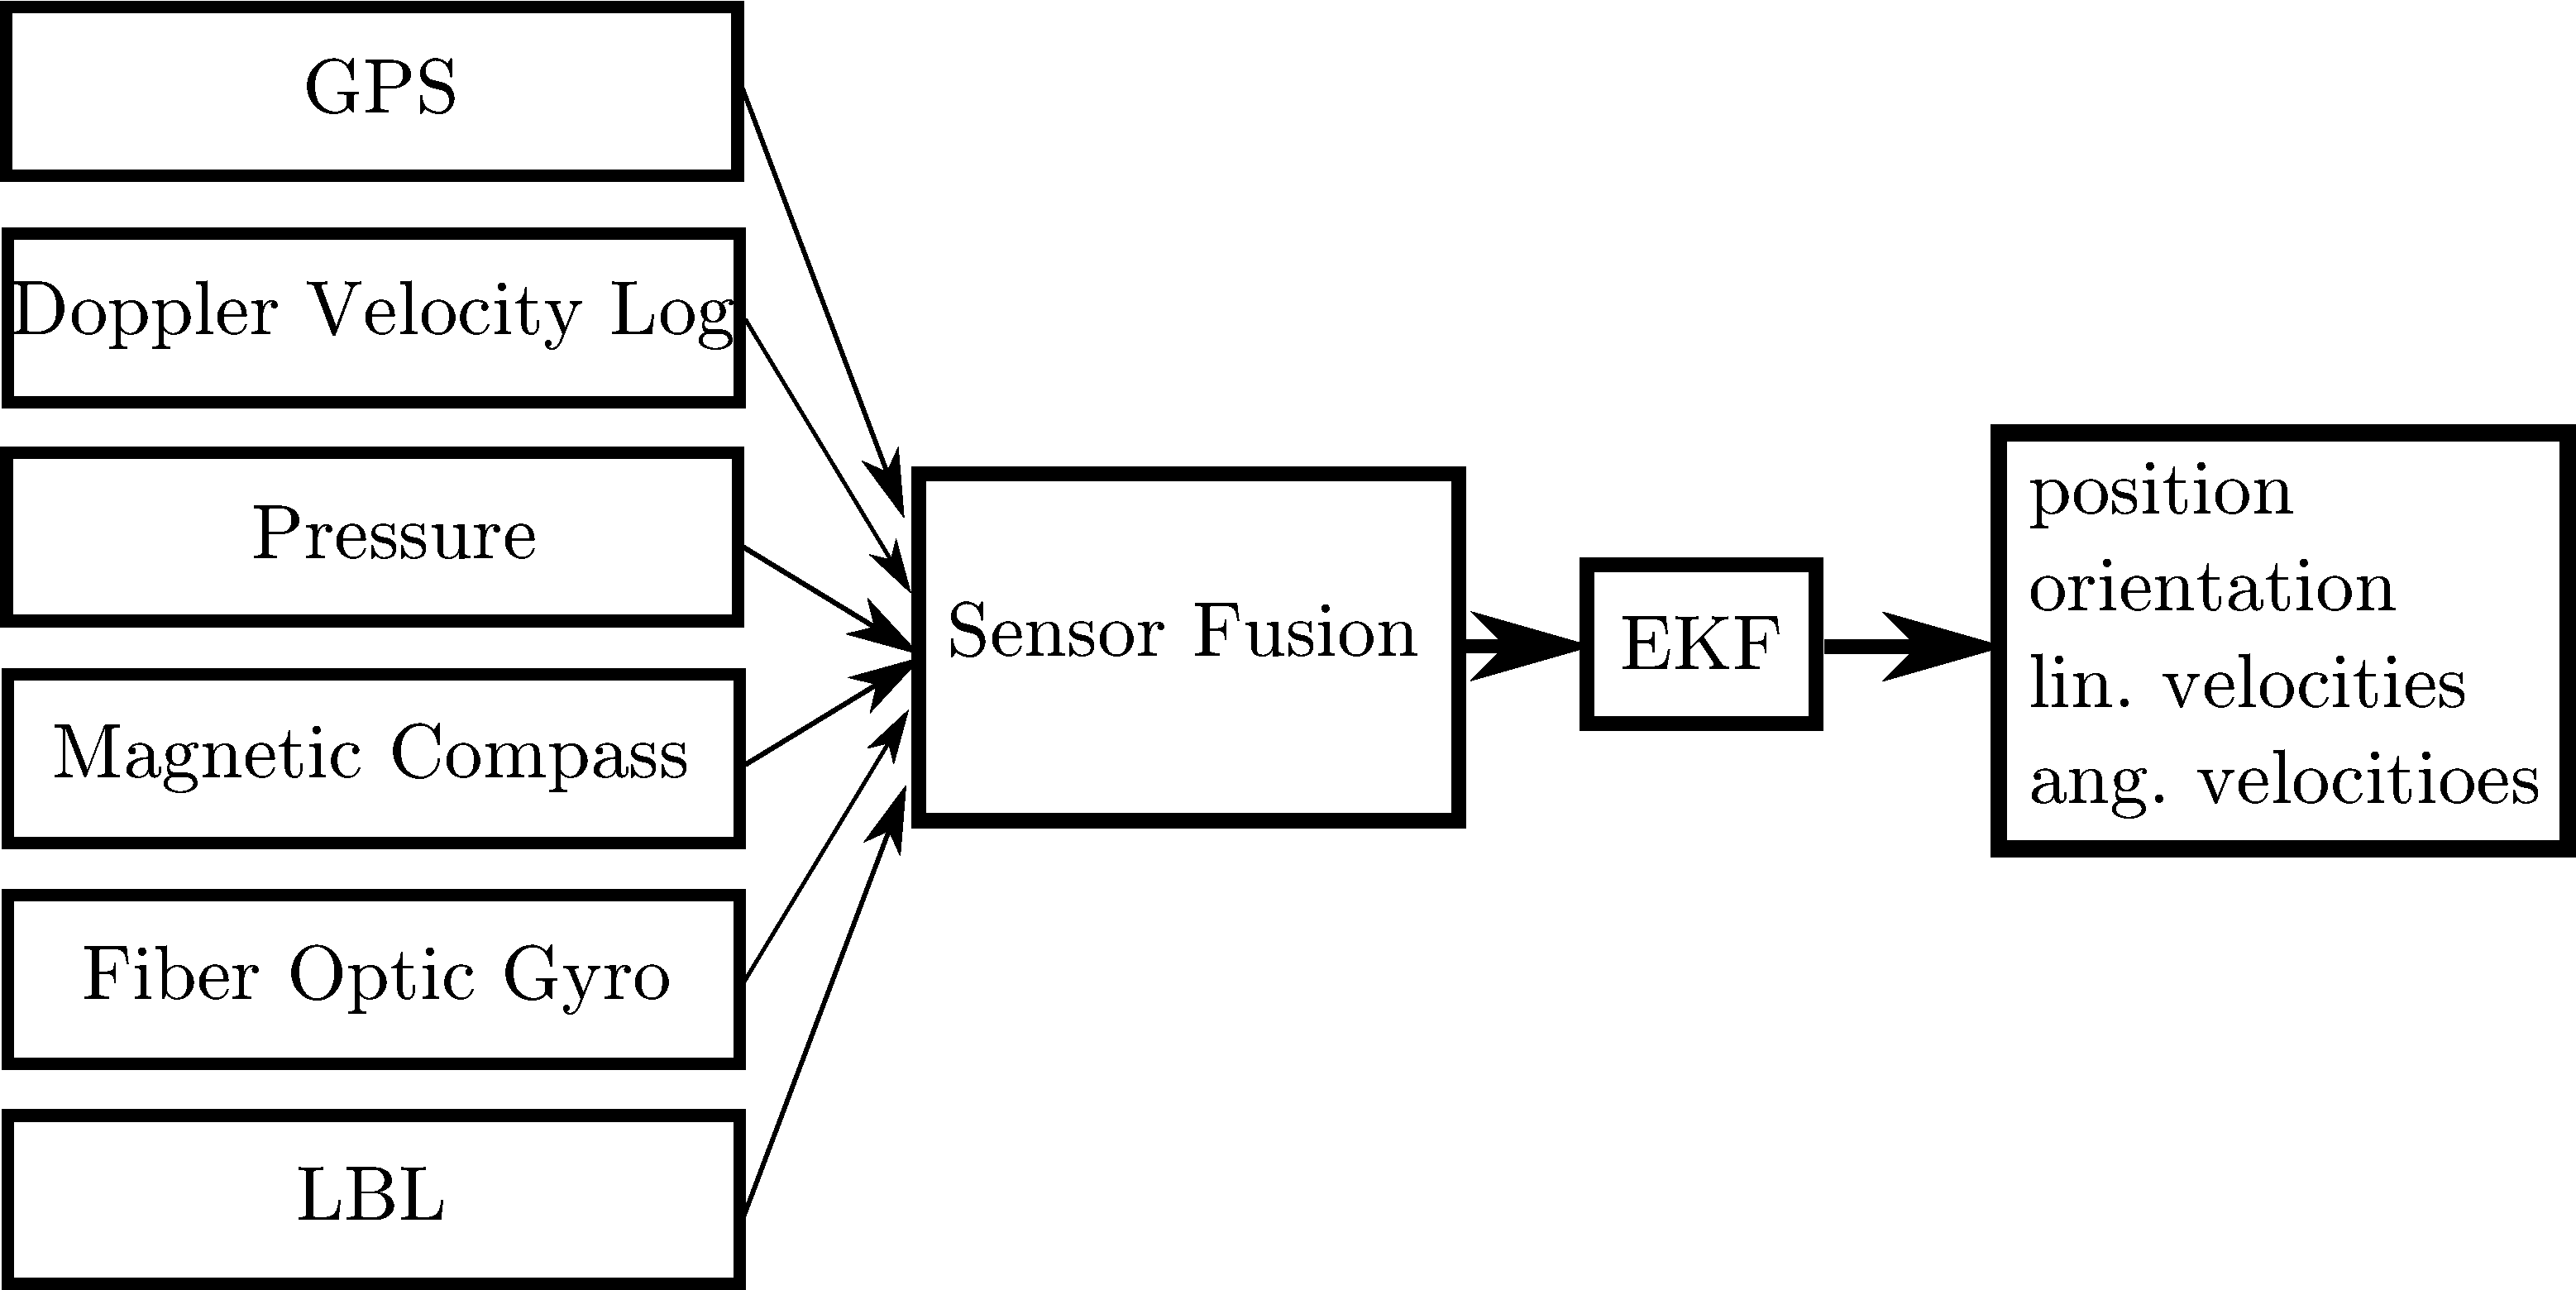
\includegraphics[width=0.4\textwidth]{fusion.pdf}
  \caption{Sensor fusion diagram.}
\vspace{-10pt}
\label{fig:sensor-fusion}
\end{figure}
EKF fuses the measurements from all the devices together: localisation algorithm collects the incoming sensor information and computes the pose of the vehicle by filtering the data cluster obtained from sensor devices. Such procedure is regarded as \textit{sensor fusion} (Figure ~\ref{fig:sensor-fusion}). Basic sort of sensor fusion implementation is incorporated in navigation algorithm by combining different quantities into a jointly updated state vector with position, orientation and velocities (\S~\ref{sec:implementation}).
%%%%%%%%%%%%%%%%%%%%%%%%%%%%%%%%%%%%%%%%%%%%%%%%%%%%%%%%%%%%%%%%%%%%%%%%%%%%%%%%
\section{IMPLEMENTATION}  \label{sec:implementation}
\begin{figure}%[htb]
  \centering
    \subfigure[AUV positioning - global frame of reference.] {\label{fig:auv-positioning}
	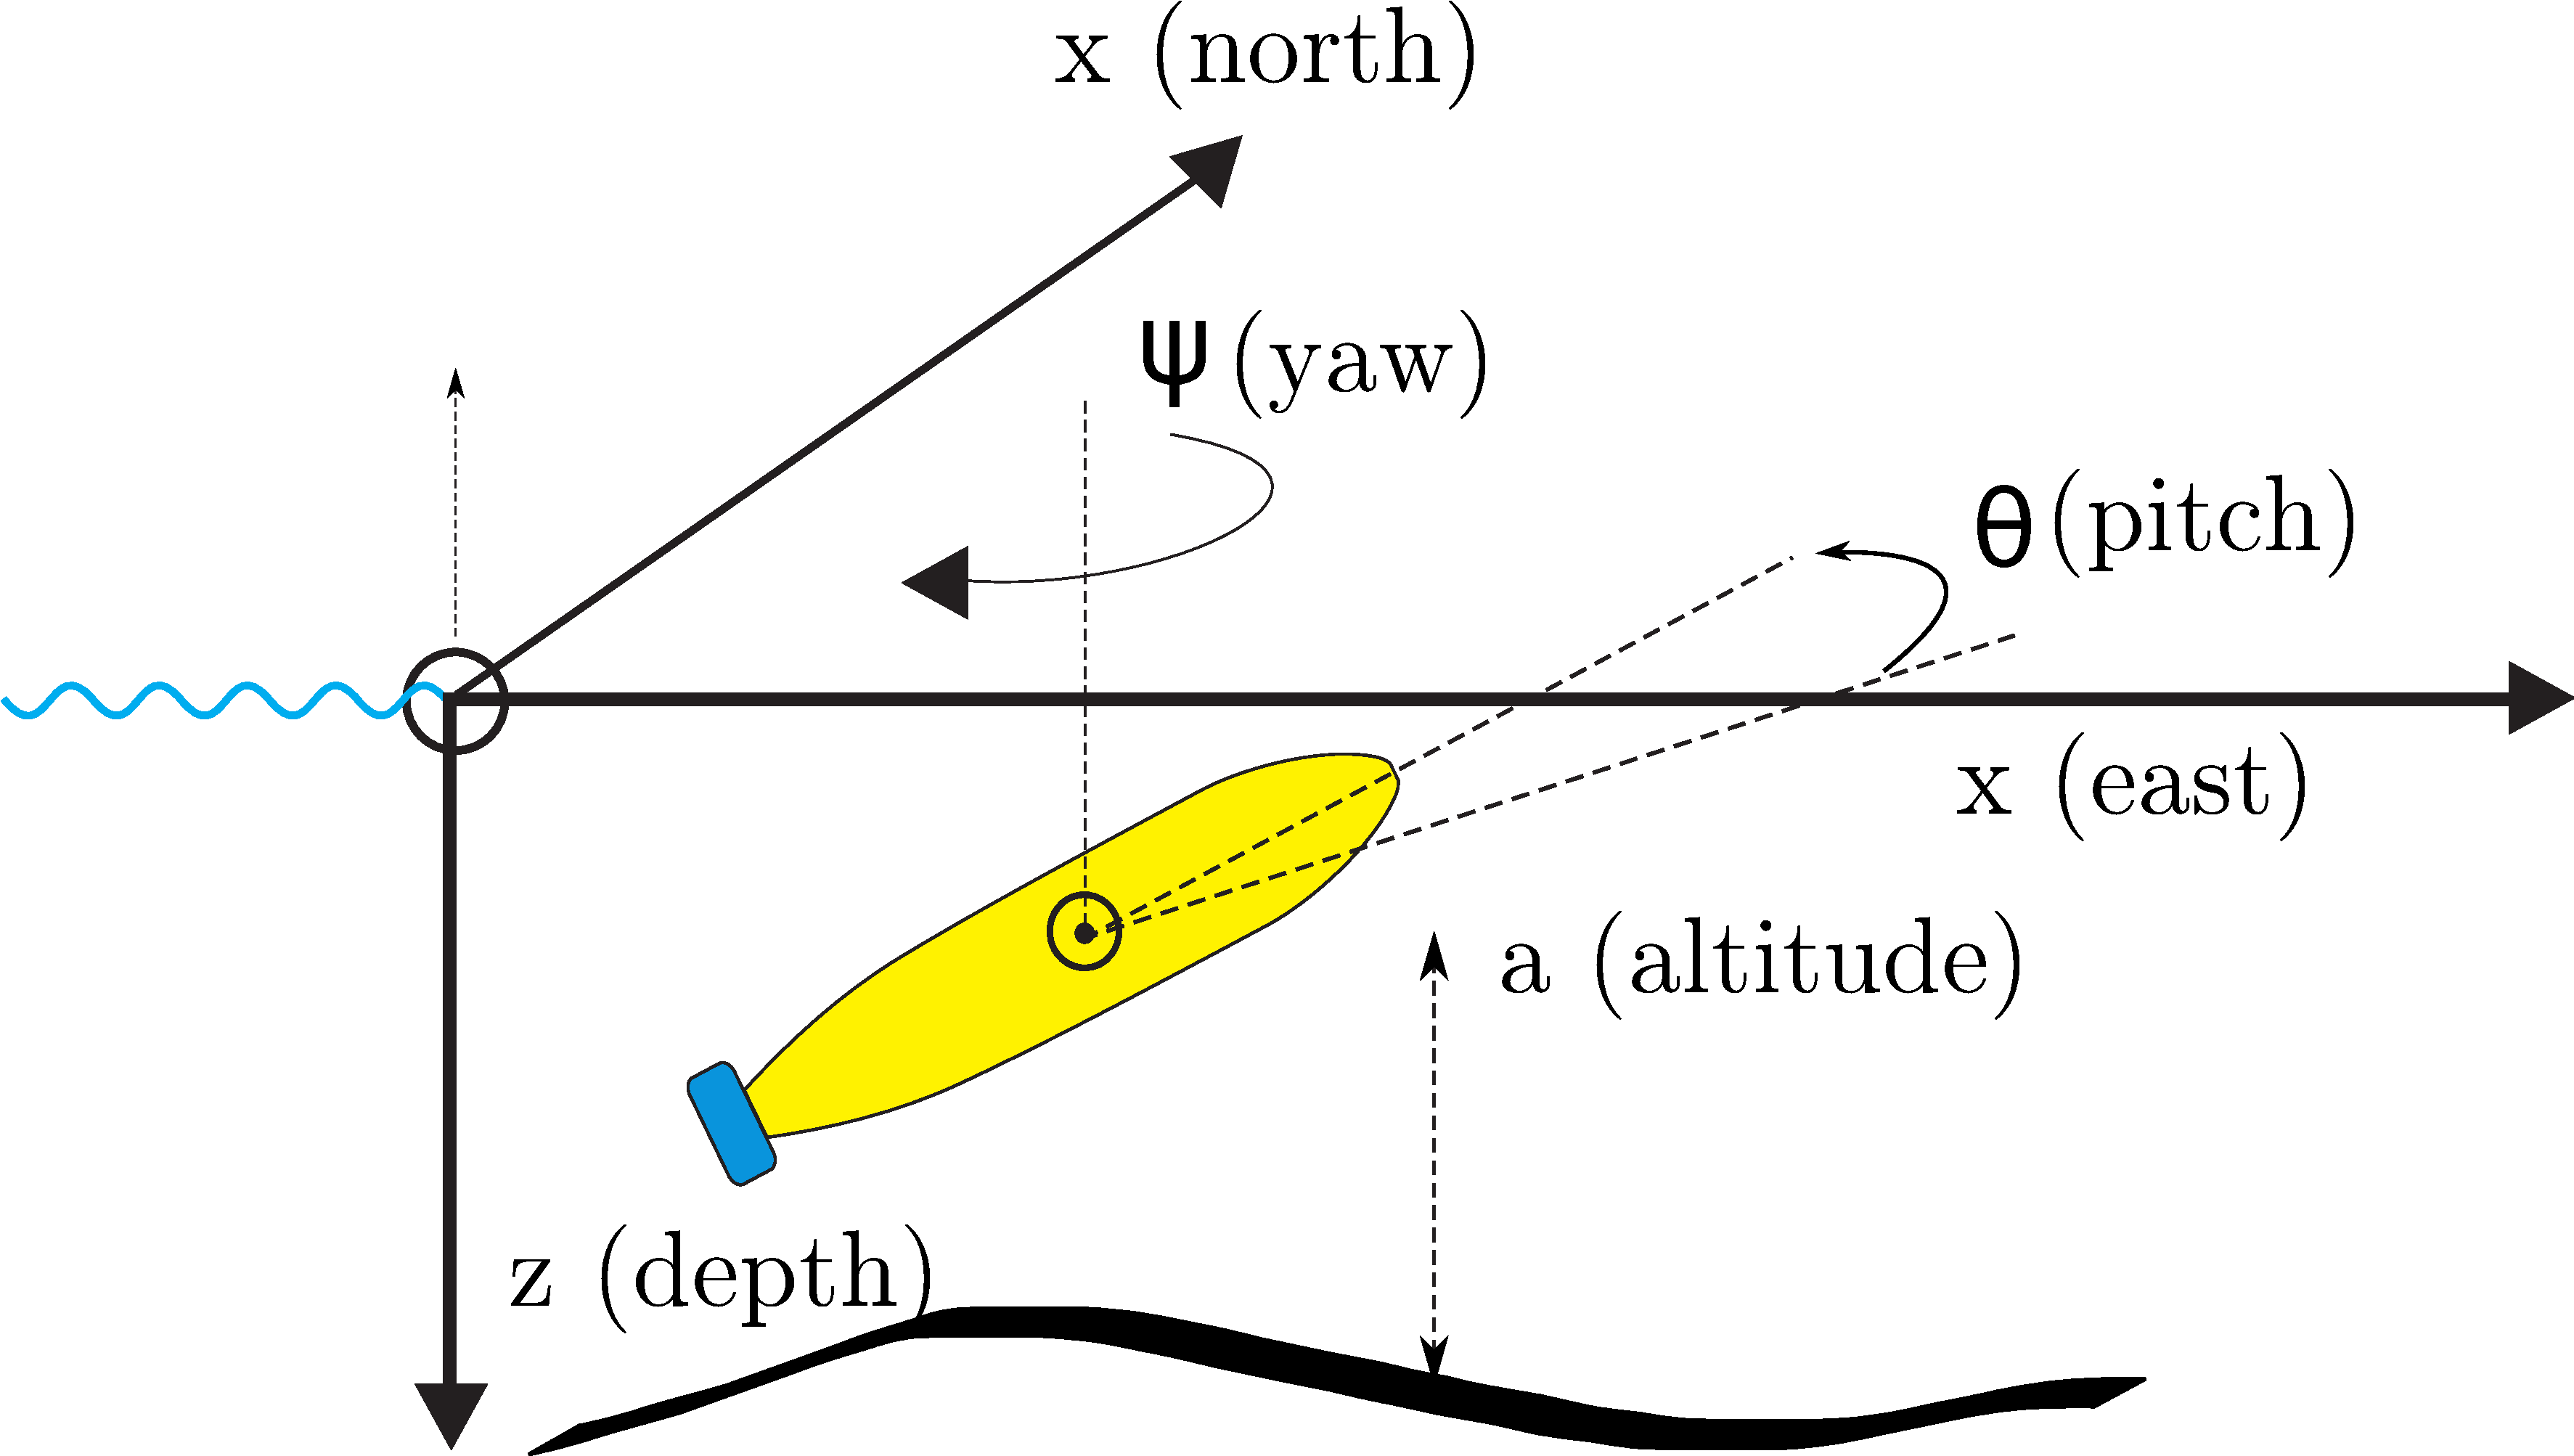
\includegraphics[width=0.8\linewidth]{auv-model.pdf}} \\
    \subfigure[AUV body frame - local coordinate system with movement directions.] {\label{fig:auv-axes}
    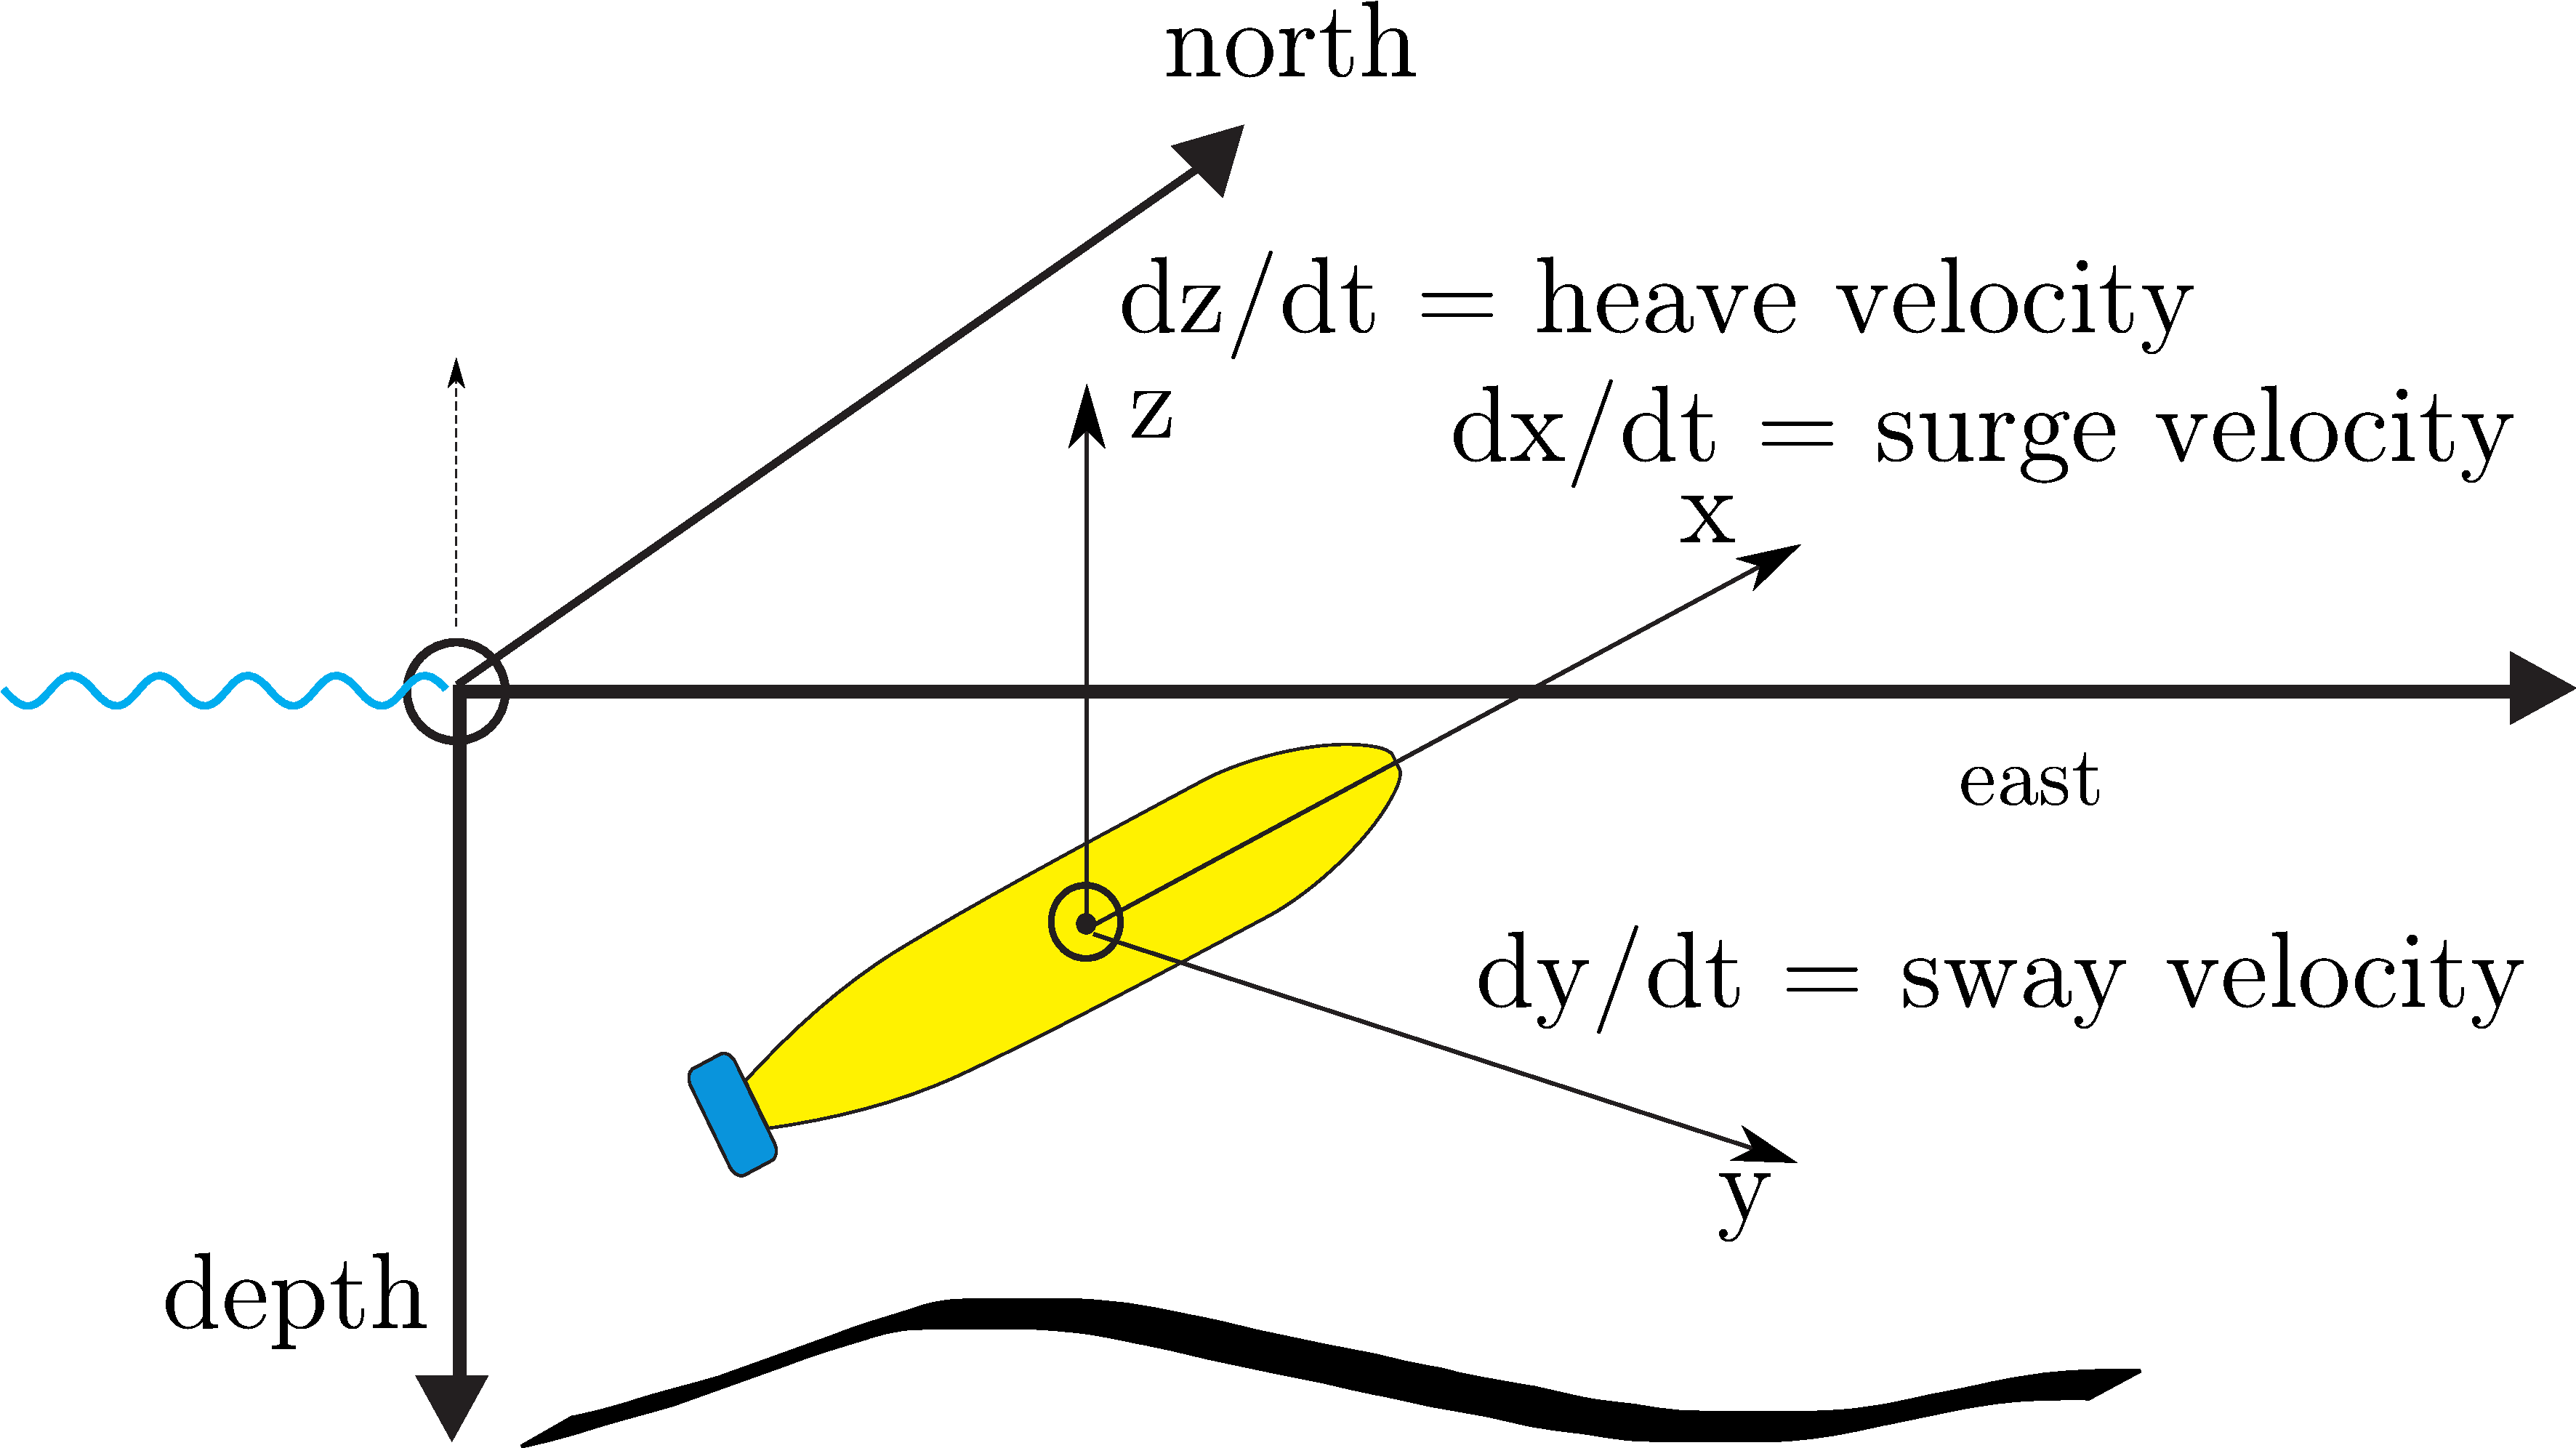
\includegraphics[width=0.8\linewidth]{auv-axes.pdf}}
\caption{AUV state vector values and five degrees of freedom.}
\label{fig:auv-states}
\vspace{-10pt}
\end{figure}
Position, orientation and velocities of a vehicle underwater are stored within the state vector. Proposed solution for localisation uses state-space approach and EKF to estimate the value of the state vector using data from odometry sensors and acoustic positioning system (LBL), if available. Reasons for choosing this method are influenced by the application itself. Localisation is intended to work in unstructured environments, with no clear visibility, relying on kinetic and absolute position measurements.
%Data are merged together using the EKF. 
Mathematical model of the system is the integral part of the EKF. It is used to define the state transition law by applying well known kinematic equations which describe object motion \cite{thrun05}. \textit{Constant velocity} 5DOF kinematic model is used as system model to predict the movements of the submerged body \cite{ribas10}. States are predicted at each time-step using the model $f()$ and previous state $\vect{X}(k-1)$ (equation ~\ref{eq:state-tran}).
\begin{equation}
\vect{X}(k) = f(\vect{X}(k-1), \vect{N}(k-1))
\label{eq:state-tran}
\end{equation}

\textit{Process model} is used to describe the state transition in time. In proposed discrete-time stochastic model, 5DOF include position values and two angle states: yaw and pitch - making altogether five possible values to change in modelling vehicle position (figure ~\ref{fig:auv-positioning}). Since the application uses state-space approach, focus will be on defining a state vector that would incorporate all the relevant values for the dynamic system - kinematic and position variables. In spirit of that, system state vector combines together metric and angular values. At discrete time moment $k$, it values:
$$ \vect{X}(k) = 
\left[ 
\begin{array}{ccccccccccc}
x & y & z & a & u & v & w & \psi & \varphi & \dot{\psi} & \dot{\varphi}
\end{array}
\right] ^{T} $$  
$x$ takes the value of \textit{north} (expressed in meters), $y$ is \textit{east} and $z$ is \textit{depth}. $a$ marks the \textit{altitude} with $u$, $v$ and $w$ standing for linear velocities: \textit{surge}, \textit{sway} and \textit{heave velocity}, respectfully. The rest of the state vector covers angular values (expressed in radians or degrees). $\psi$ and $\varphi$ are used as yaw and pitch, hence describing the vehicle orientation. $\dot{\psi}$ and $\dot{\varphi}$ are angular velocities: yaw rate and pitch rate, respectfully. The state vector incorporates all the relevant information necessary to describe the system under investigation. Angle and velocity for pitch degree of freedom is included in 5DOF system model since it can make a difference in estimating vehicle location in cases of tilted vehicle movement. Model uses previous state and noise to make a prediction on the next state vector value $\vect{X}(k)$  using non-linear function $f()$ and process noise vector $\vect{N}$ (Equation ~\ref{eq:state-tran}) where $\vect{N} = \left[ \begin{array}{ccccc} \dot{u} & \dot{v} & \dot{w} & \ddot{\psi} & \ddot{\varphi} \end{array} \right]^{T}$. Process noise models inaccuracies or unpredictable disturbances in motion model \cite{ristic04}. 
\begin{figure*}%[ht!]
\vspace{-10pt}
%\hrulefill
\begin{equation}
\label{eq:state-tran-matrix}
\begin{bmatrix} x \\ y \\ z \\ a \\ u \\ v \\ w \\ \psi \\ \varphi \\ \dot{\psi} \\ \dot{\varphi} \end{bmatrix}_{(k)} =
\begin{bmatrix} x + (uT+\dot{u}\frac{T^{2}}{2})\cos(\psi)\cos(\varphi) - (vT+\dot{v}\frac{T^{2}}{2})\sin(\psi)\cos(\varphi) \\ 
                y + (uT+\dot{u}\frac{T^{2}}{2})\sin(\psi)\cos(\varphi) + (vT+\dot{v}\frac{T^{2}}{2})\cos(\psi)\cos(\varphi) \\ 
                z + (wT+\dot{w}\frac{T^{2}}{2})\cos(\varphi) \\ 
                a - (wT+\dot{w}\frac{T^{2}}{2})\cos(\varphi) \\ 
                u + \dot{u}T \\ 
                v + \dot{v}T \\ 
                w + \dot{w}T \\ 
                \psi    + \dot{\psi}T    + \ddot{\psi}   \frac{T^{2}}{2} \\ 
                \varphi + \dot{\varphi}T + \ddot{\varphi}\frac{T^{2}}{2} \\ 
                \dot{\psi}    + \ddot{\psi}T \\ 
                \dot{\varphi} + \ddot{\varphi}T
\end{bmatrix}_{(k-1)} 
\end{equation}
%\hrulefill
\vspace{-10pt}
\end{figure*}
To summarize, implementing vehicle localization using EKF demands establishing two models: first one describing the state evolution (\textit{system model}) and the second model that associates noisy measurement with the state (\textit{measurement model}). 

EKF (\S~\ref{sec:ekf}) was chosen for the state estimation as a logic choice being an algorithm that integrates together different sensor measurements, makes a sub-optimal, recursive state estimation and above all, is derived for nonlinear systems \cite{thrun05}. The main feature of EKF is that it linearises the system model and measurement model nonlinear functions. System model is further developed according to formulas ~\ref{eq:der-proc-state}, ~\ref{eq:der-proc-noise}, ~\ref{eq:der-mes-state} and ~\ref{eq:der-mes-noise}.

Knowing plant model and deriving $\vect{F}(k)$, $\vect{W}(k)$ enables EKF algorithm to complete the prediction stage using known formulas. Next step is the correction of the prediction using data obtained from measurement.
\begin{figure}%[htp]
  \begin{center}
    \subfigure[EKF filters after each sensor measurement.]   {\label{fig:asynch}   
    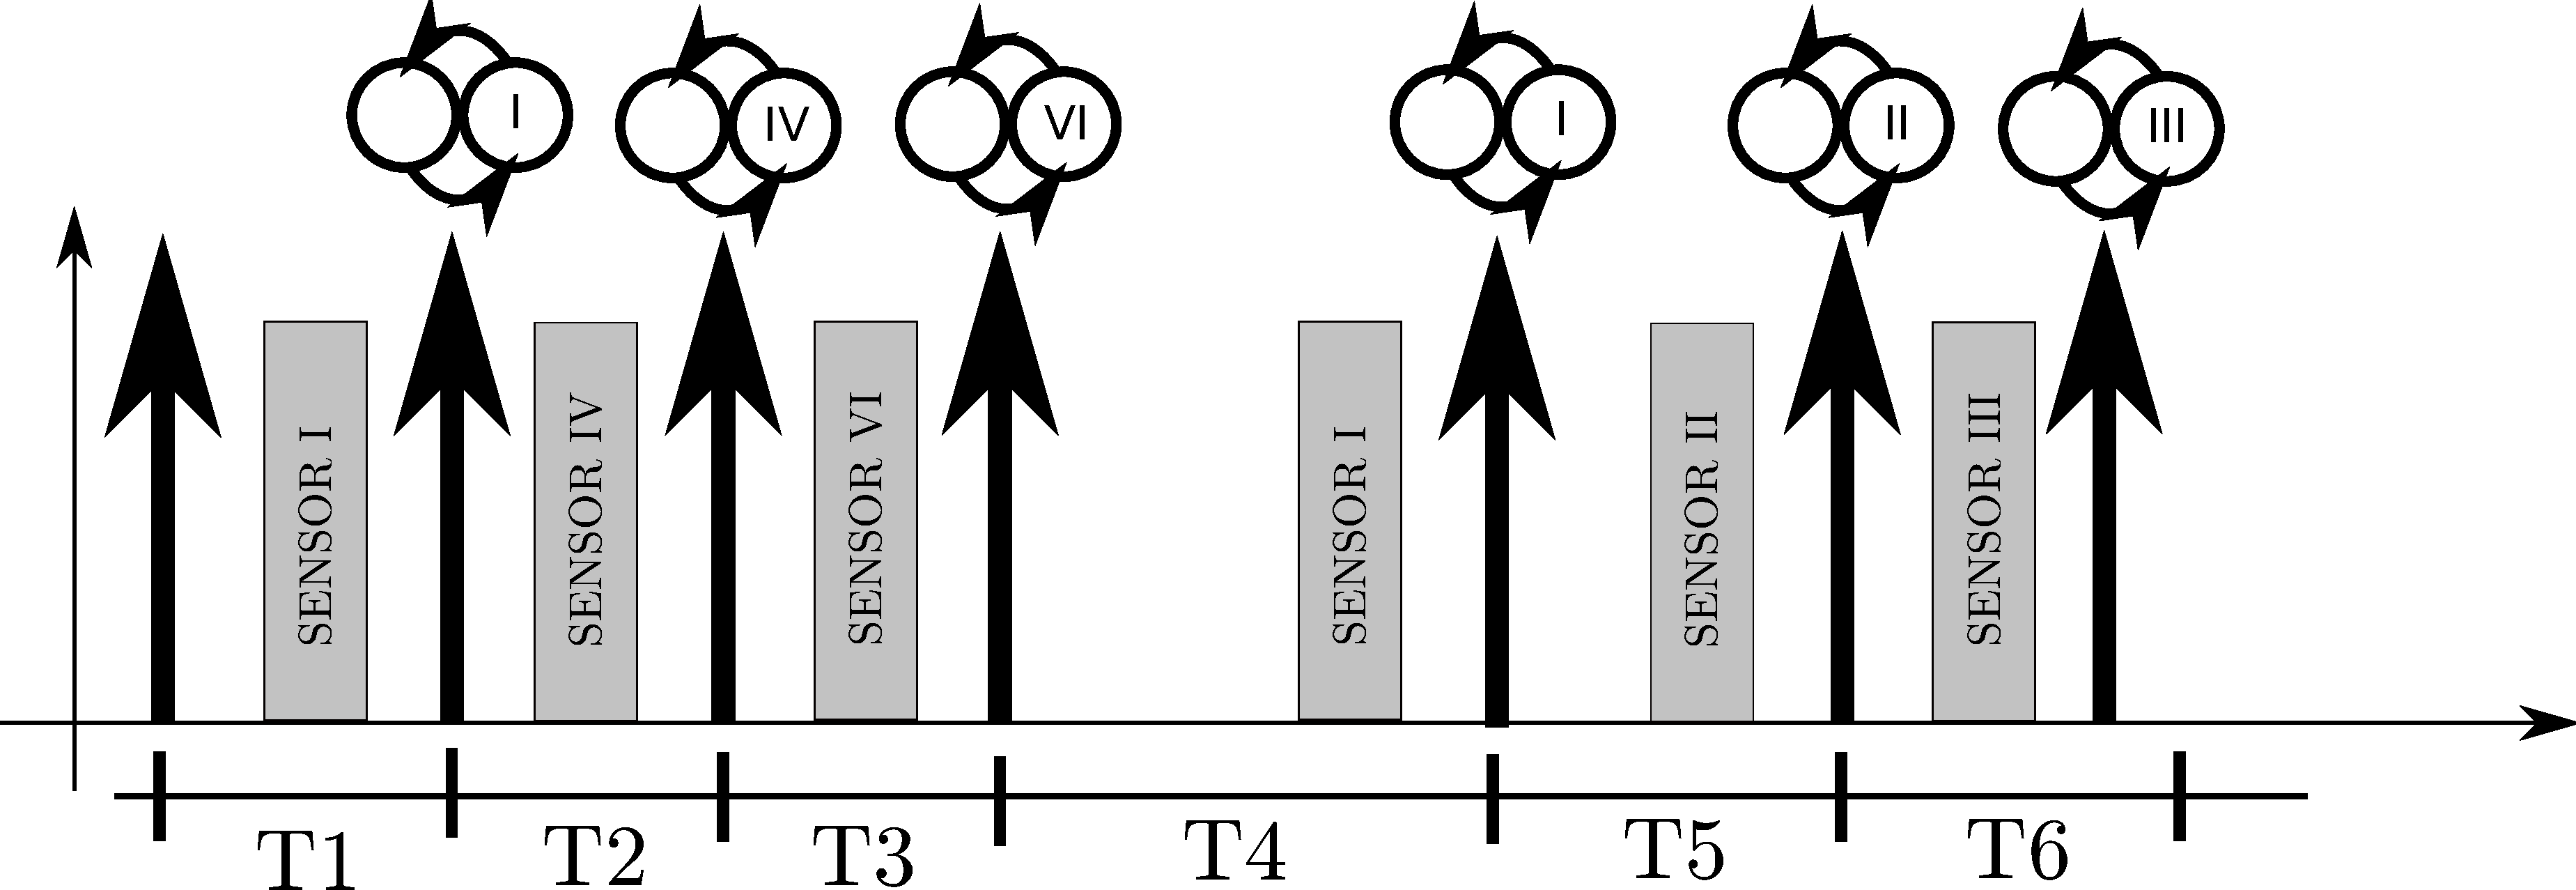
\includegraphics[width=0.4\textwidth]{asynch.pdf}}
    \subfigure[EKF filters periodically.]{\label{fig:synch}
    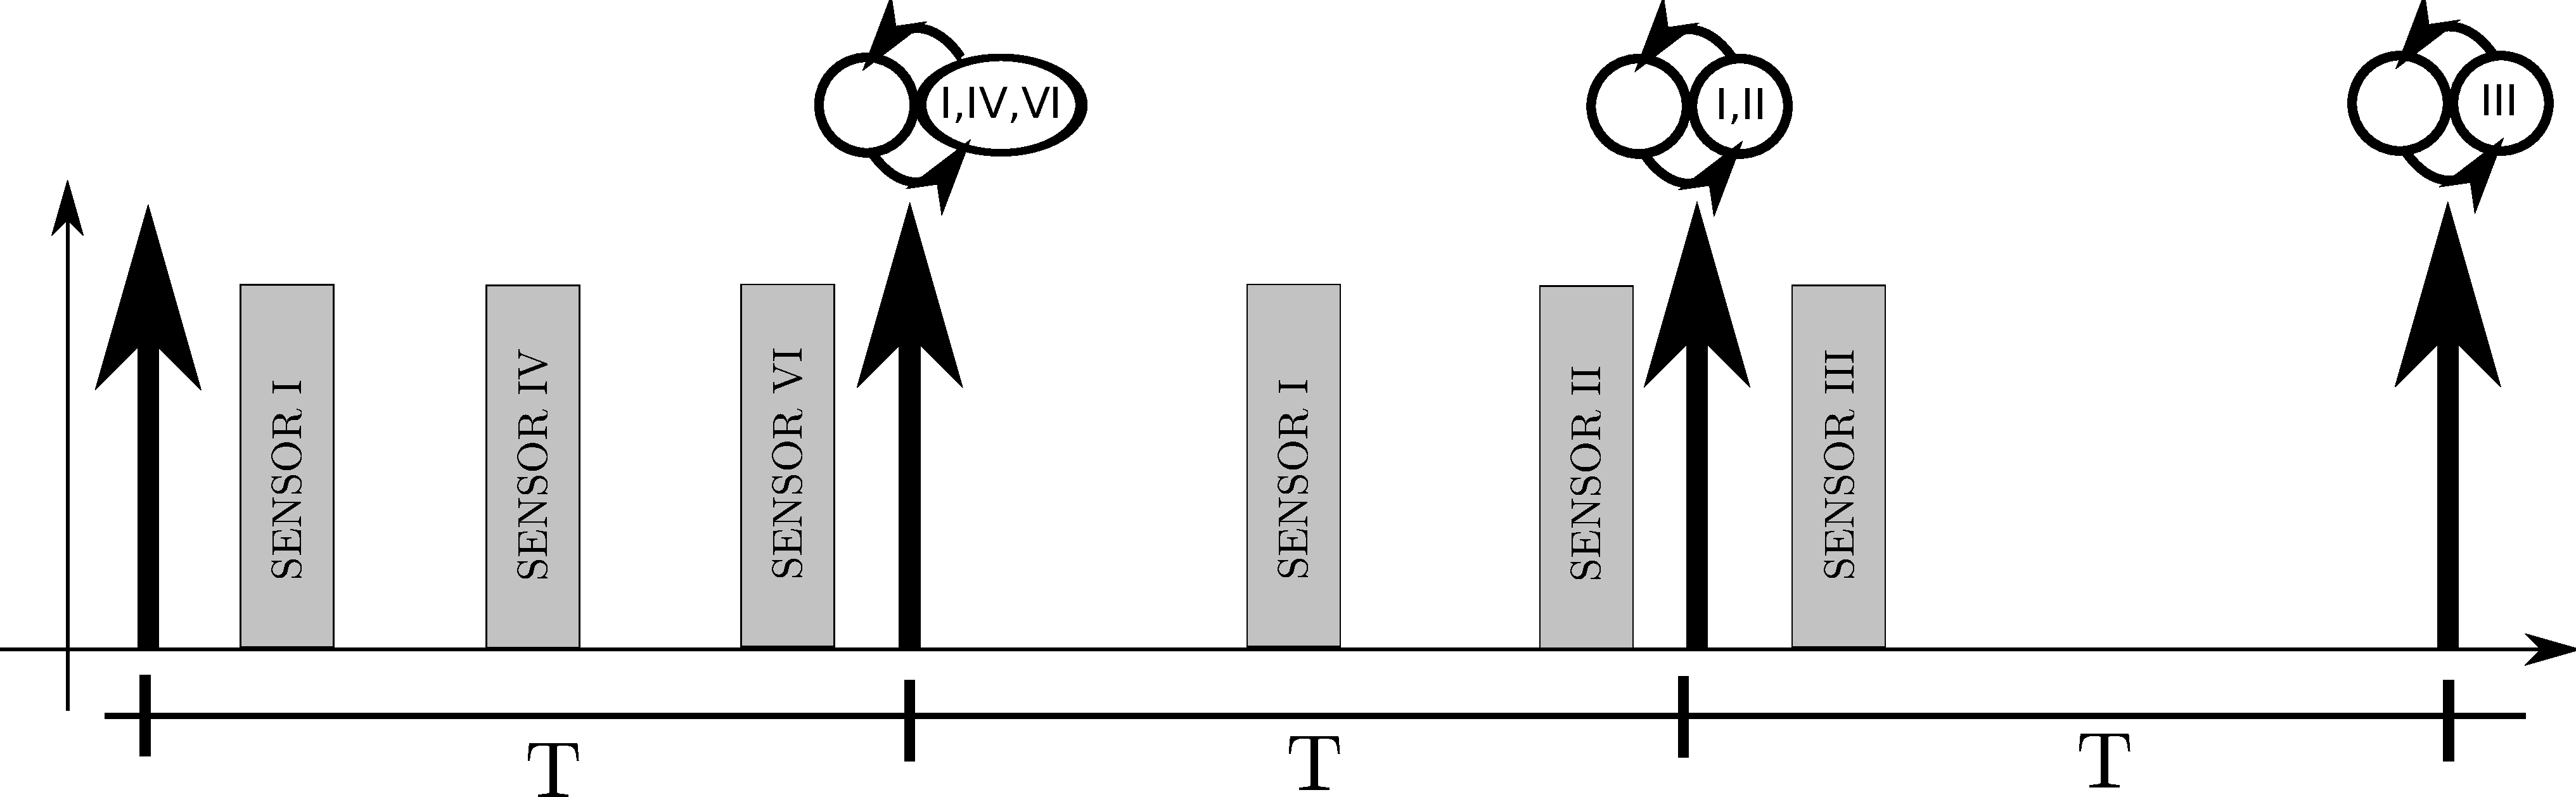
\includegraphics[width=0.4\textwidth]{synch.pdf}}  
  \end{center}
  \caption{Two modes for combining together sensor measurements into observation.}
  \vspace{-10pt}
  \label{fig:ekf-modes}
\end{figure}
\textit{Measurement model} introduces measurement equation which establishes the connection between the measurements and the target state (equation ~\ref{eq:mes-model}) where $Z(k)$ represents the measurement at time $k$, $X(k)$ represents state vector and $M(k)$ represents noise. Purpose of the measurement is to be able to update, correct the state $X(k)$ using measurements $Z(k)$. $h()$ is generally a non-linear function. EKF linearises the measurement model.
\begin{equation}
\vect{Z}(k) = h(\vect{X}(k), \vect{M}(k)) = \vect{H} \vect{X}(k \mid k-1)  + \vect{M}(k)
\label{eq:mes-model}
\end{equation}
%$h()$ can be expressed with matrix containing ``ones'' at particular positions since
For this particular application and available sensor configuration, state vector elements are measured directly, hence the measurement relation becomes equality. There is no need for partial derivation (Equation ~\ref{eq:mes-model}). Measurement noise is submitted in form of an additive Gaussian zero-mean noise assigned to each measured value. Measurement (observation) noise is characterised with zero mean $(E \lbrace \vect{M}(k) \rbrace = \vect{0})$ and standard deviation $(E \lbrace \vect{M}(k) \vect{M}^{T}(k) \rbrace)$ given as diagonal covariance matrix with diagonal elements set to constant filter parameter $\sigma^{2}$ for each of the measured values (Figure ~\ref{eq:concatenate-mes}). It expresses how much we trust in the measurement, how uncertain or varying measurement of each of the state values is. 

One of the features of the process is that measurements are not available all the time. The reason is the nature of the process of estimating the location itself. Simply - messages from sensors arrive at different moments and it happens that some of the sensors could not be available due to different causes (no ``dvl lock'', for instance). The idea is to take all the available information periodically and integrate it together in measurement model, as a filter observation (Figure ~\ref{fig:synch}). Alternatively, each message can be filtered upon its arrival (Figure ~\ref{fig:asynch}). In case observation is empty, filter does the prediction only. Idea for the solution has been introduced in \cite{ribas10}. Some other implementations of EKF for underwater navigation have reported the usage of similar strategy for merging the measurements together \cite{drolet00, blain03}. This way, measurement model adopts to the set of the values observed.

Integrating together several different sensor-specific measurements into one observation would imply concatenating together several measurement matrices $(\vect{Z}, \vect{H})$ and measurement noise matrices $(\vect{R})$, as shown in ~\ref{eq:concatenate-mes} for the sample case of two sensor device measurements included in one observation. EKF maintains its own timer for the observations (value T from the model). As an example, depth sensor measures depth $(z)$ and heave velocity $(w)$, thus $$\vect{Z}_{depth} =\left[\begin{array}{cc} z & w \end{array} \right] ^{T}$$, $$\vect{H}_{depth} =\left[\begin{array}{ccccccccccc} 0 & 0 & 1 & 0 & 0 & 0 & 0 & 0 & 0 & 0 & 0 \\ 0 & 0 & 0 & 0 & 0 & 0 & 1 & 0 & 0 & 0 & 0 \end{array} \right]$$ and $$\vect{R}_{depth} =\left[\begin{array}{cc} \sigma_{depth}^{2} & 0 \\ 0 & \sigma_{w}^{2} \end{array} \right] $$. Where $\sigma$ marks the standard deviation expressing how much we trust in  measurement. It is given as EKF parameter. Similar pattern values for the other sensors depending on values that they measure.
\begin{figure*}
\begin{equation}
\label{eq:concatenate-mes} 
\vect{Z}(k) = \left[ \begin{array}{c} \vect{Z}_{sensor I} \\ \vect{Z}_{sensor II}  \end{array} \right],
\vect{H}(k) = \left[ \begin{array}{c} \vect{H}_{sensor I} \\ \vect{H}_{sensor II}  \end{array} \right], 
\vect{R}(k) = \left[ \begin{array}{ccc} \vect{R}_{sensor I} & 0 \\ 0 & \vect{R}_{sensor II} \end{array} \right]
\end{equation}
\vspace{-10pt}
\end{figure*}
%\\ \vect{Z}_{sensor III} \\ \vect{H}_{sensor III}  & 0  & 0    \\ 0 & 0 & \vect{R}_{sensor III}
Having more than one measurement involved in estimation of the global state is a good characteristic. The estimate which uses more diverse data gives better estimate since it is possible to combine together more that one sort of observation. Another advantage follows the fact that the whole set of state variables is updated each time, resulting in more correlation between variables. Hence those that are missing for some reason can be compensated this way. Results of simulations using authentic data and the  real missions are given in Section \S~\ref{sec:results}. Odometry integrates velocity and acceleration data collected from devices such as gyroscope or accelerometers. Integration of noisy data over time or usage of ``relative measurements'' (those calculated from absolute measurements) results in drift or bias of the final estimate. In order to recover from that, algorithms perform the correction. Correction takes an absolute measurement which should be less precise, possibly noisy, but not prone to drifting. %An example which illustrates the phenomenon could be a man that walks with the eyes closed trying to keep the track of his position by measuring the steps and predicting where he could possibly be judging on number of steps and their size. Steps have the role of ``relative measurement'' - one quantity is used to estimate the other one that's correlated with it. Naturally, a man will keep making errors in his position estimate. Moreover, these errors will accumulate over time producing drift. Correction would require the man to open his eyes and observe the current position (absolute measurement), compare it with the position predicted by counting steps and neutralise the drift before carrying on with the eyes closed. 
%%%%%%%%%%%%%%%%%%%%%%%%%%%%%%%%%%%%%%%%%%%%%%%%%%%%%%%%%%%%%%%%%%%%%%%%%%%%%%%%
\chapter{Results} \label{chap:results}
Main purpose of the thesis is the implementation of a navigation system that uses measurements from different sensors, fuses the sensory data together in order to make presumably better quality estimate of the position and the orientation of the underwater robot. Existing data from the real missions were used to carry out the initial trials. It is useful to mention that there is no exact ground truth for underwater robot localization available. GPS signal, if available, could serve as an absolute position reference: either directly or in form of LBL. Experimental results have been obtained for different missions. Good news, however, is that the absolute depth measurement is quite accurate and frequent, making AUV localisation a 2D task.  

\section{Real navigation scenario} \label{sec:real-scenario}
Authentic data taken from previously recorded Nessie mission were used to simulate the algorithm ``offline'' as the part of the stage intended for testing and correcting. Besides, being able to repeat the same measurement scenario enables more insight in filtering process and benefits of fusing together the sensor data. \textit{.bag} files (\url{http://www.ros.org/wiki/}) containing recorded real-time messages with sensor measurements, were used as source. Furthermore, it allows designing the code in its original C++ form that will require little modification once deployed on the vehicle in form of ROS package since \textit{.bag} files emulate authentic messages and timestamps. One of the deficiencies of the evaluation of localisation results is the fact that there is no exact ground truth to compare the result with. Dead reckoning localisation substituted with occasional LBL position updates was compared with the localisation obtained after filtering (Figures ~\ref{fig:auv-sim-straight2}, ~\ref{fig:auv-sim-straight1}) for the recorded straight line trajectory mission. 

\T{Selecting a heading measurement with good performance}
For a high-end underwater vehicle such as Nessie, supplied with FOG-based INS, DVL and LBL, main source of navigation error is influenced by transformation of vehicle-referenced velocities to world-referenced velocities \cite{bahr08}, particularly due to yaw (heading) measurement errors. Yaw can be measured using several devices, each having different accuracy and performance. Simulation with data from previous missions was carried out to see which device gives the best performance for a given underwater vehicle. 

Heading calculated by integrating FOG's yaw rate - tends to be accurate and fast, less prone to noise. Nevertheless, it is calculated each time by appending yaw rate value integrated in time on the previous yaw value (relative measurement). Therefore, it is sensible on initial absolute heading measurement. In case initial yaw is imprecise, a constant bias exists in yaw measurement (Figure ~\ref{fig:auv-sim-straight1}). Constant bias causes sudden steps in position estimate obtained using EKF. This is expected scenario since the sensor responsible for measuring initial heading is magnetic compass, device sensitive to disturbances coming from environment (Figure ~\ref{fig:magnetic-disturb}). In real experiments biggest obstacle was proper calibration of magnetic compass. In practice, tests have showed many failures in compass heading measurement, possibly due to calibration and magnetic declination. There is yet space to do more testing with better compass tuning. To overcome the problem of accurate yaw measurement, EKF used in experiments will either ignore the yaw measurement (it is possible since sensor fusion successfully compensates missing heading information with yaw rate obtained from FOG) or use it with high variance assigned to yaw measurement. 
%Finally, initial heading is given with magnetic compass.

\T{Loch Earn dataset - straight line movement}: Example of basic EKF localisation using inertial measurements aided with LBL acoustic positioning system was tested on straight line movement of approximately 80 m length, recorded at the lake Loch Earn. For simulation purposes, sensor measurements are stored in a \textit{.bag} file, that can be replayed, producing real-time messages of sensor measurements as they originally occurred. At this point, it is important to revise which sensors were used, their main features and, finally, filtering parameters. 

Standard sensor configuration comprising of pressure sensor, magnetic compass, FOG and DVL is used in the mission. Absolute position correction was carried out using LBL system. Important fact is that the heading was measured with magnetic compass only at the beginning. Later on, it kept being calculated by integrating yaw rate obtained from FOG. Alternative solution for the heading measurement would be the usage of compass for direct acquiring of yaw, but such option exposed calibration difficulties. Result of EKF localisation algorithm was shown in north-east map (Figure ~\ref{fig:sim-straight2}, ~\ref{fig:sim-straight1}). Different parameter values for EKF were tested. Table ~\ref{tab:ekf-params} revises all filter parameters used for filter tuning, together with their role. Essentially, setting high standard deviation for a Gaussian of a certain parameter can be interpreted as having more uncertainty in value that it represents - whether it is a measurement uncertainty or uncertainty of the predicted value (model uncertainty). Therefore, we can choose to be confident in certain sensor measurement and/or certain model prediction, and observe the simulation outcome of such setting. Setting the parameters properly improves the performance of the filter.  
\addtocounter{footnote}{1}
\footnotetext[\value{footnote}]{as it appears in algorithm equations}  
\begin{table*}
\centering
	\caption{EKF navigation parameters.}
	\label{tab:ekf-params}
\begin{tabular}{llll}
\toprule
Parameter      &     Signature $^{\decimal{footnote}}$     &     Units     &    Description  \\
\midrule
                         & \multicolumn{3}{c}{standard deviation of the ... } \\ 
\multirow{1}{*}{SDNorth} & \multirow{1}{*}{$\sigma_{n}$} & \multirow{1}{*}{$m$} & \multirow{1}{*}{north observation} \\
\multirow{1}{*}{SDEast}  & \multirow{1}{*}{$\sigma_{e}$} & \multirow{1}{*}{$m$} & \multirow{1}{*}{east observation} \\
\multirow{1}{*}{SDDepth} & \multirow{1}{*}{$\sigma_{d}$} & \multirow{1}{*}{$m$} & \multirow{1}{*}{depth observation} \\
\multirow{1}{*}{SDAltitude} & \multirow{1}{*}{$\sigma_{a}$} & \multirow{1}{*}{$m$} & \multirow{1}{*}{altitude observation} \\
\multirow{1}{*}{SDu} & \multirow{1}{*}{$\sigma_{u}$} & \multirow{1}{*}{$\frac{m}{s}$} & \multirow{1}{*}{surge velocity observation} \\
\multirow{1}{*}{SDv} & \multirow{1}{*}{$\sigma_{v}$} & \multirow{1}{*}{$\frac{m}{s}$} & \multirow{1}{*}{sway velocity observation} \\
\multirow{1}{*}{SDw} & \multirow{1}{*}{$\sigma_{w}$} & \multirow{1}{*}{$\frac{m}{s}$} & \multirow{1}{*}{heave velocity observation} \\
\multirow{1}{*}{SDyaw} & \multirow{1}{*}{$\sigma_{\psi}$} & \multirow{1}{*}{$rad$} & \multirow{1}{*}{heading observation} \\
\multirow{1}{*}{SDpitch} & \multirow{1}{*}{$\sigma_{\varphi}$} & \multirow{1}{*}{$rad$} & \multirow{1}{*}{pitch observation} \\
\multirow{1}{*}{SDyawRate} & \multirow{1}{*}{$\sigma_{\dot{\psi}}$} & \multirow{1}{*}{$\frac{rad}{s}$} & \multirow{1}{*}{heading rate observation} \\
\multirow{1}{*}{SDpitchRate} & \multirow{1}{*}{$\sigma_{\dot{\varphi}}$} & \multirow{1}{*}{$\frac{rad}{s}$} & \multirow{1}{*}{pitch rate observation} \\
\midrule
                         & \multicolumn{3}{c}{standard deviation of the ... process noise} \\
\multirow{1}{*}{SDuModel} & \multirow{1}{*}{$\sigma_{\dot{u}}$}  & \multirow{1}{*}{$\frac{m}{s^{2}}$} & \multirow{1}{*}{surge acceleration} \\
\multirow{1}{*}{SDvModel} & \multirow{1}{*}{$\sigma_{\dot{v}}$}  & \multirow{1}{*}{$\frac{m}{s^{2}}$} & \multirow{1}{*}{sway acceleration} \\
\multirow{1}{*}{SDwModel} & \multirow{1}{*}{$\sigma_{\dot{w}}$}  & \multirow{1}{*}{$\frac{m}{s^{2}}$} & \multirow{1}{*}{heave acceleration} \\
\multirow{1}{*}{SDyawRateModel} & \multirow{1}{*}{$\sigma_{\dot{v}}$}  & \multirow{1}{*}{$\frac{rad}{s^{2}}$} & \multirow{1}{*}{yaw acceleration} \\
\multirow{1}{*}{SDpitchRateModel} & \multirow{1}{*}{$\sigma_{\dot{w}}$}  & \multirow{1}{*}{$\frac{rad}{s^{2}}$} & \multirow{1}{*}{pitch acceleration} \\
\bottomrule
\end{tabular} 
\end{table*}
Straight line movement with authentic sensor measurements recorded in Loch Earn was a basis for initial tests of the EKF localisation algorithm. Red line shows the dead reckoning navigation, which is directly updated with absolute position update (LBL). Dead reckoning uses values periodically ($\approx$5$Hz$) obtained from DVL and FOG (linear velocities: $u$ and $v$ and heading $\psi$, respectfully), and substitutes them into equations similar to ones used for north and east prediction within prediction model: 
$$ north = north + (uT+\dot{u}\frac{T^{2}}{2})\cos(\psi) - (vT+\dot{v}\frac{T^{2}}{2})\sin(\psi) $$
$$ east  = east  + (uT+\dot{u}\frac{T^{2}}{2})\sin(\psi) + (vT+\dot{v}\frac{T^{2}}{2})\cos(\psi) $$
% SDnorth/east = 5 $cm$, 
% SDnorth/east = 5 $cm$, 
\begin{figure}%[htb]
  \centering
    \subfigure[N/E localisation. Yaw was calculated by integrating yaw rate periodically measured using FOG.] {\label{fig:sim-straight2}
	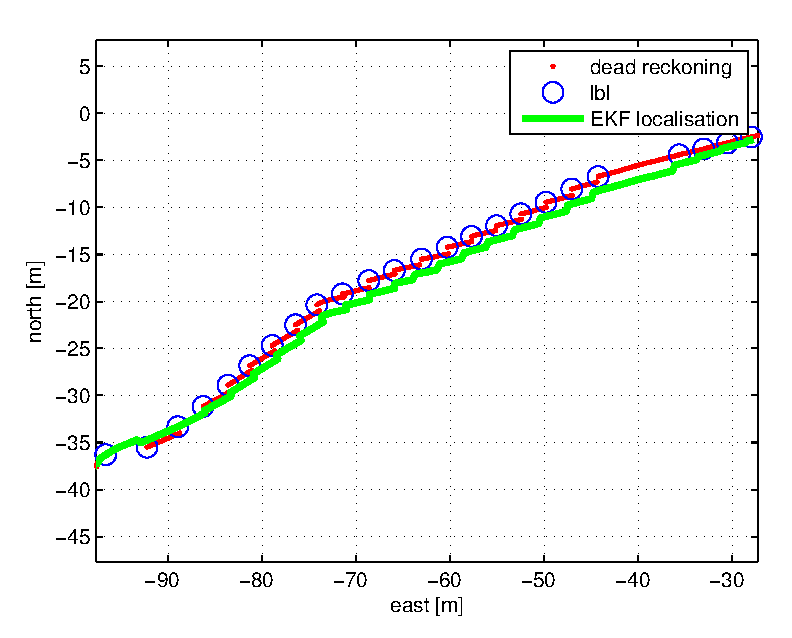
\includegraphics[width=0.48\linewidth]{simulations/fig/sim-straight2.eps}}
    \subfigure[Heading estimation. Biased yaw measurement not being corrected due to high confidence in yaw measurement.] {\label{fig:yaw-straight2}
    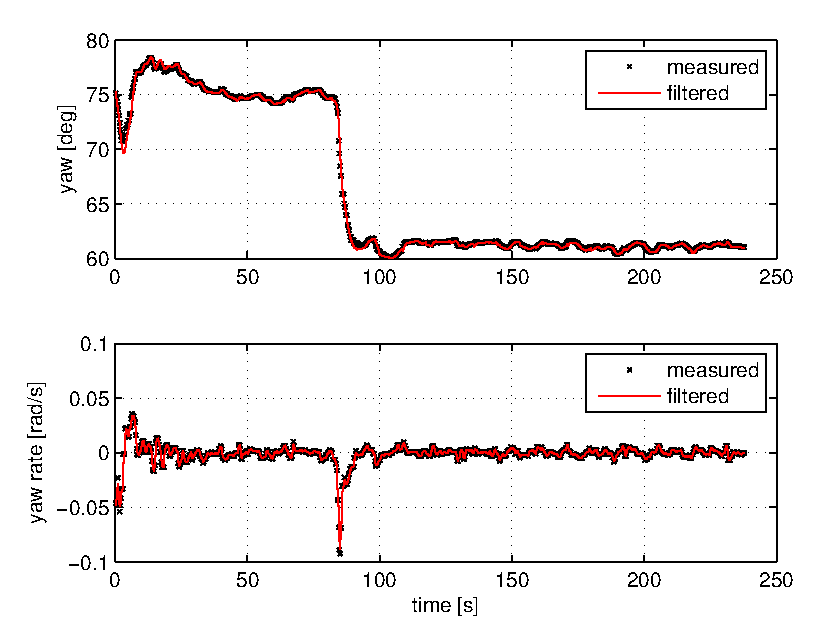
\includegraphics[width=0.48\linewidth]{simulations/fig/yaw-straight2.eps}} \\   
\caption{AUV localisation using EKF with high confidence in yaw measurement, SDyaw = 0.01$rad \approx 0.6 ^{\circ}$. SDyawRate = 0.004 $\frac{rad}{s}$, SDu/v = $1\frac{cm}{s}$.}

\label{fig:auv-sim-straight2}
\end{figure}
\begin{figure}%[htb]
  \centering
    \subfigure[N/E localisation. Yaw was calculated by integrating yaw rate periodically measured using FOG.] {\label{fig:sim-straight1}
	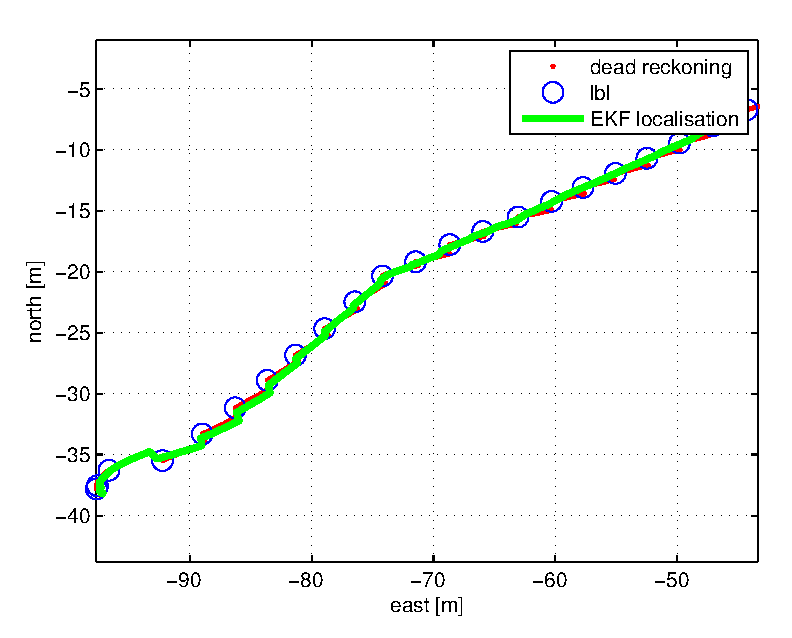
\includegraphics[width=0.48\linewidth]{simulations/fig/sim-straight1.eps}}
    \subfigure[Heading estimation. Biased yaw measurement is being corrected.] {\label{fig:yaw-straight1}
    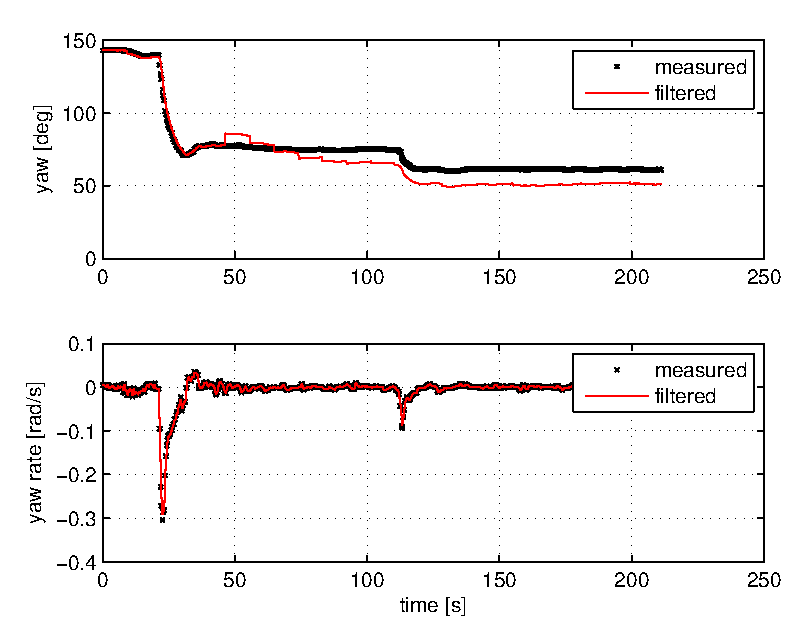
\includegraphics[width=0.48\linewidth]{simulations/fig/yaw-straight1.eps}} \\
\caption{AUV localisation using EKF with low confidence in yaw measurement, SDyaw = 0.2$rad \approx 11.5 ^{\circ}$. SDyawRate = 0.004 $\frac{rad}{s}$, SDu/v = $1\frac{cm}{s}$.}
%\vspace{-10pt}
\label{fig:auv-sim-straight1}
\end{figure}    
%After  initial heading, yaw rate was integrated in time to calculate yaw.    when setting  EKF parameter uncertainty  when using EKF, this time
EKF updates periodically (synchronous mode), with period set to 230 ms. At first, simulation parameters \textit{SDnorth}, \textit{SDeast}, \textit{SDyaw} and \textit{SDyawRate} were set to low values - suggesting high trust in measurements. Resulting trajectory (Figure ~\ref{fig:sim-straight2}) shows that the heading measurement has a constant bias, caused by the error in initial heading measurement obtained by compass. Thus, yaw measurement, calculated relative to previous value each time, propagates the error (bias). Biased yaw observation further on causes EKF localisation to experience sharp jumps. To overcome this using EKF framework, less confidence was assigned to the yaw measurement (\textit{SDyaw}) value. Eventually, bias becomes visible if measured and filtered heading are compared (Figure ~\ref{fig:yaw-straight1}). As for the rest of the heading information, rate of yaw measurement will be incorporated with a lot of confidence (\textit{SDyawRate} parameter having range of degrees) since it is a reliable device and it does not depend on the initial estimate. Good feature of sensor fusion is that lack of one measurement or its low performance can be compensated with some other measurement considering that they are combined together in mathematical model in the right manner. In case of yaw and yaw rate - the derivation in time is a relation that connects them together. 

Simulation shows that localisation performance can be tailored by setting the confidence in prediction model or measurement values. Confidence is materialized as standard deviation (variance) of the random variable: the lower it is, more certain the value of the random variable is hence more confident in value of that variable we tend to be. Kalman filter tries to optimise the result within the defined boundaries of uncertainty. 

Unscented Kalman filter was mentioned in Section \S~\ref{sec:ukf} as a good alternative in handling nonlinearities. UKF was implemented in MATLAB for the simulation purposes and its result compared with the EKF localisation, under same parameter settings and using the real data obtained from Nessie sensors. Test mission consisted of pipe tracking where the vehicle was guided along the underwater pipe three times and each time returned back to the initial position (Figure ~\ref{fig:ekf-ukf}). 2D north-east maps were compared, together with dead reckoning, same as one used for previous simulations. General characteristics of UKF are visible from the obtained shape of the UKF path (Figure ~\ref{fig:ekf-ukf}). Eventually, both filtered paths end up in approximately same position, having less drift than the dead reckoning. EKF does first order approximations, therefore, its path is slightly distorted compared with the UKF one, which was obtained with the same amount of calculation, and the inherited approximation of at least second order \cite{julier96}. Simultaneously with filtering, UKF preserves the nonlinearity formula of prediction model better - its curves have shape closer to equation-based dead reckoning curves. Still, a question that is yet opened is whether we need to improve the approximation of the prediction model. Answering this question is a hard task without knowing the movement of the object and how much it actually matches the state prediction model. A difficulty with UKF implementation is that it involves calculation of covariance matrix square root which is a slightly more complex problem, solved with numerical methods. Nevertheless, it is possible that covariance matrix becomes singular which also depends on parameter $k$ used for scaling (Section \S~\ref{sec:ukf}). $k$ was set to -0.5 for simulations shown.        
\begin{figure}%[htb]
  \centering
    \subfigure[N/E localisation. Comparison of the EKF and UKF.] {\label{fig:ekf-ukf}
	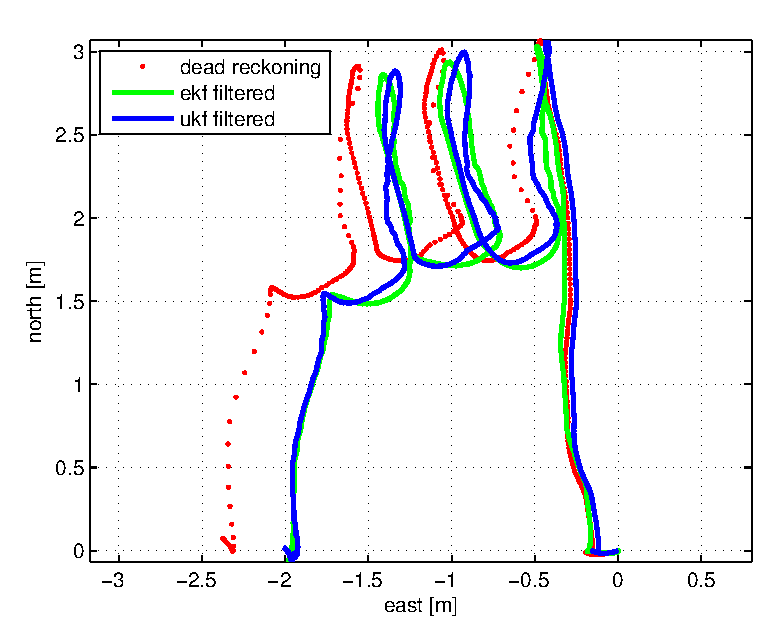
\includegraphics[width=0.42\linewidth]{simulations/fig/UKFpipeTrack.eps}}
    \subfigure[Magnetic disturbances affecting the heading measurement by compass. Vehicle is not moving, FOG is not oscillating at the same time.] {\label{fig:magnetic-disturb}
    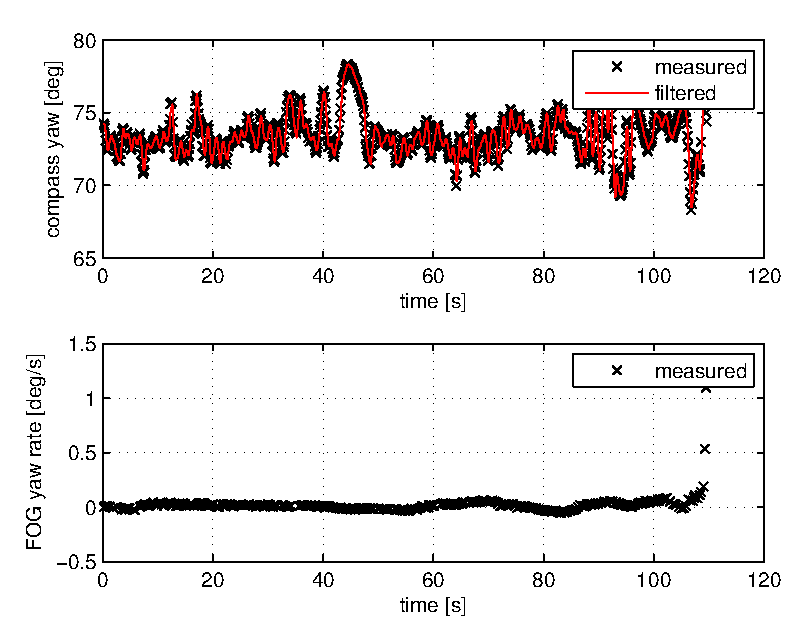
\includegraphics[width=0.42\linewidth]{simulations/fig/magnetic.eps}} 
%\vspace{-33pt}  
\end{figure}

\T{Sensor fusion for heading: } being in search for heading measurement less prone to initial error, and guided by simulation results, real scenarios were accomplished using magnetic compass for heading measurement. Compass is more sensitive to magnetic disturbances (Figure ~\ref{fig:magnetic-disturb}), slower than FOG but, importantly, gives an absolute measure. Therefore, it does not rely on previous measurements. An experiment was made by just manually rotating the robot horizontally while keeping the same position - changing its heading. Figures ~\ref{fig:lostFog} and ~\ref{fig:lostCompass} show the performance of yaw filtering using EKF and the example of sensor fusion of compass and FOG. Namely, compass (Figure ~\ref{fig:lostCompass}) or FOG (Figure ~\ref{fig:lostFog}) were disabled at one point during the experiment. When one of them stops working, the other one tries to compensate the failure. 
%and still filters the heading/yaw rate variation.  
\begin{figure}%[htb]
  \centering
    \subfigure[Compass disabled.] {\label{fig:lostCompass}
	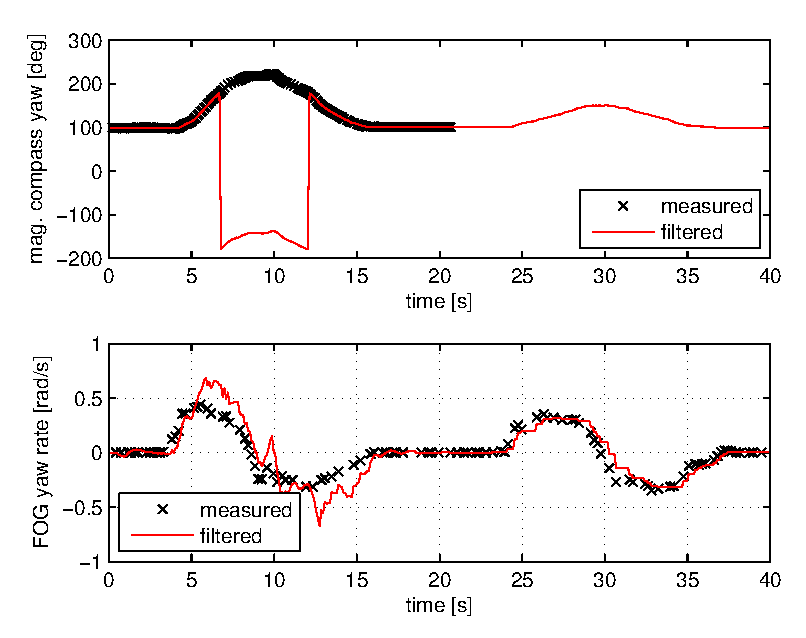
\includegraphics[width=0.45\linewidth]{results/fig/lostCompass.eps}}
    \subfigure[FOG disabled.] {\label{fig:lostFog}
    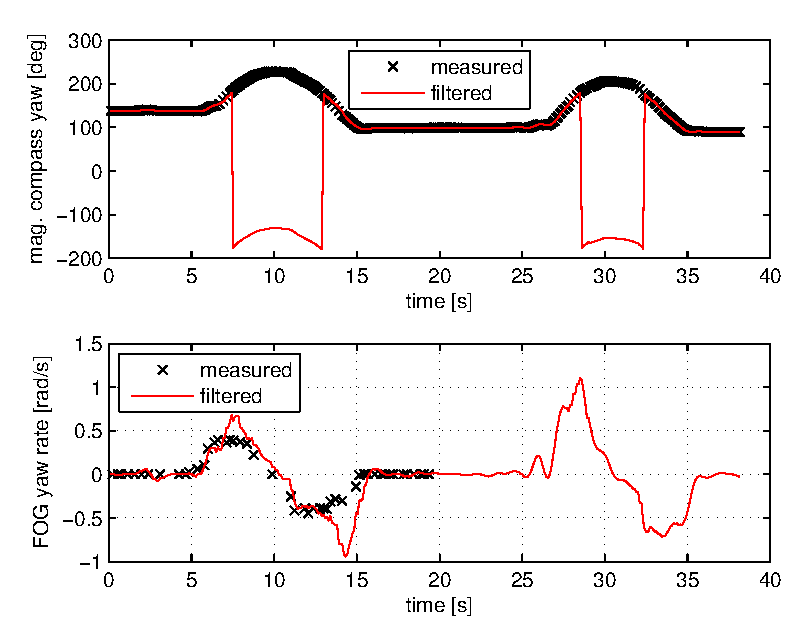
\includegraphics[width=0.45\linewidth]{results/fig/lostFOG.eps}} \\   
\end{figure}

\T{Trajectory filtering: } Spiral trajectory and surfacing action was taken with Nessie starting from the depth of around 12 m. EKF filtering results are shown in Figure ~\ref{fig:spiral} together with LBL position updates and dead reckoning starting from each position. Similarly as with previous plots, dead reckoning was shown together with LBL position updates. Filtered trajectory does not experience severe jumps, and the curve seems to be smoother and less prone to drifting. Standard deviation of north and east measurement parameter (Table ~\ref{tab:ekf-params}) was tested with different values, causing more or less confidence in LBL measurement hence shaping the filtered localisation curve. Presented LBL measurements are exhibiting quite diverse range of values.

Causes of position correction errors are numerous: from ``multipathing'' outliers (Figure ~\ref{fig:multipathing}) till the imprecision inferred from the nature of volatile acoustic and GPS information. ``Multipathing'' causes outliers in position information as a result of false reflections for instance. Acoustic and GPS imprecision can be treated as Gaussian random variable. 
\begin{wrapfigure}{r}{0.55\textwidth}
\vspace{-10pt}
  \centering
    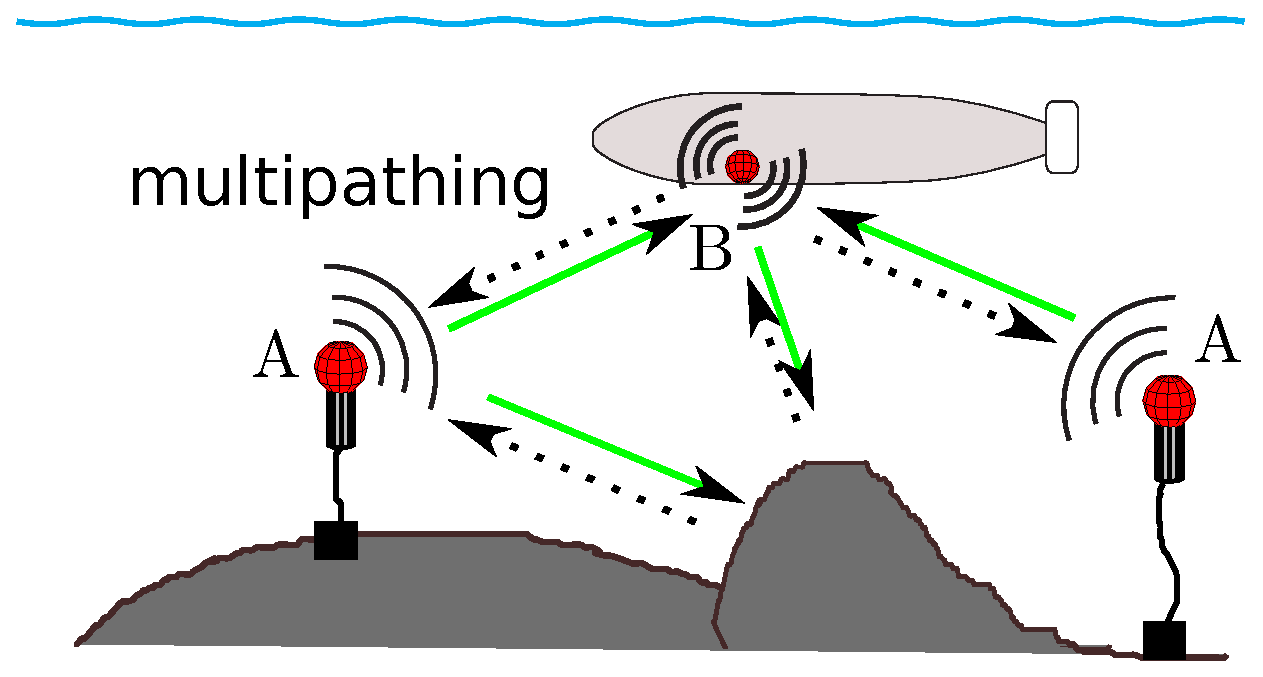
\includegraphics[width=0.45\textwidth]{results/fig/multipathing.eps}
  \caption{Multipathing can cause outliers in LBL position measurement. Due to reflection, several distances are detected, some  being false measurements.}
%\vspace{-10pt} 
\label{fig:multipathing}
\end{wrapfigure}
It is likely that some of the LBL position updates deviate from the trajectory. Hence, a mechanism for rejecting the outliers was investigated. EKF was tested on raw LBL position updates. Intention is to manage the filtration of the ``outliers'' by using properly tuned EKF. Motivation to explore such possibility comes from two scenarios encountered in earlier missions. In such missions position wad dead reckoned and LBL was used to assign each time a new value of north and east coordinate. LBL outliers were ruled out using a median filter applied on the last eleven position coordinates once the latest LBL exceeded the set threshold in position change. The missions showcased situations when: 
\begin{itemize}
\item LBL rejection is carried out despite being a ``false alarm'' - Figure ~\ref{fig:straight-median-ekf},
\item rejection of the LBL is the right choice - Figure ~\ref{fig:spiral-median-ekf}
\end{itemize}
It is important to say that LBL position filtering was implemented in form of median filter. EKF was updated with raw LBL data instead of median filter. Rejecting an LBL measurement can turn out to be right (Figure ~\ref{fig:spiral-median-ekf}) as well as a wrong decision (Figure ~\ref{fig:straight-median-ekf}). That is why EKF was suggested as an alternative. Examples of EKF's performance are shown in both Figures ~\ref{fig:straight-median-ekf} and ~\ref{fig:spiral-median-ekf}. Solution is not as categoric as median filter. Moreover, it is more robust. By giving certain trust in LBL observation it always takes it into account. Median filter, on the other hand, can be too selective in being right or wrong. If it turns out that LBL positions do follow each other, EKF continues slowly following that direction. If the outliers are isolated, EKF successfully rules them out (Figure ~\ref{fig:spiral-median-ekf}). 
\begin{figure}%[htb]
  \centering
    \subfigure[Straight trajectory: LBL outliers erroneously rejected (red). EKF tends to recover the navigation (green).] {\label{fig:straight-median-ekf}
	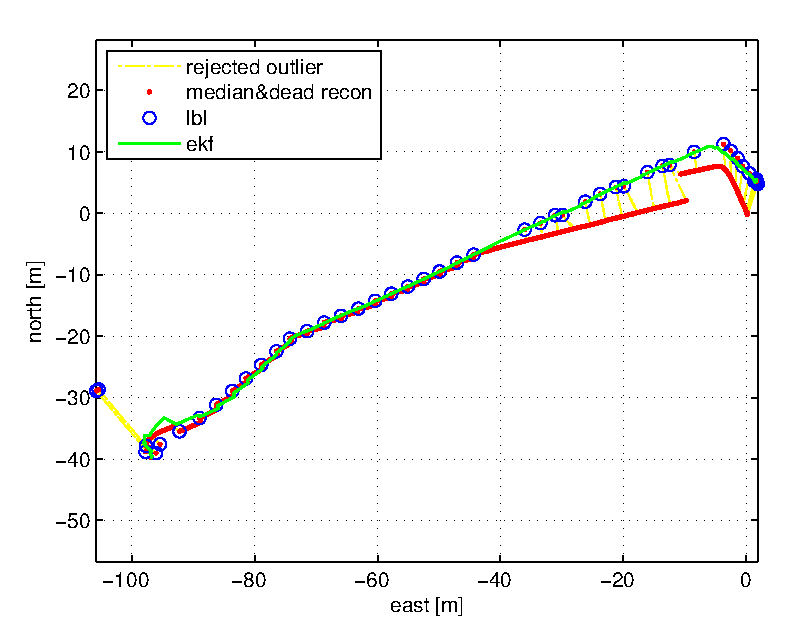
\includegraphics[width=0.47\linewidth]{results/fig/straight-median-ekf.eps}}
    %\subfigure[Straight trajectory: LBL outliers filtered with EKF.] {\label{fig:straight-ekf}
    %\includegraphics[width=0.45\linewidth]{results/fig/straight-ekf.eps}} \\  
    \subfigure[Spiral trajectory: LBL outliers are rejected using median. EKF filtering introduces the position disturbance which recovers soon after.] {\label{fig:spiral-median-ekf}
    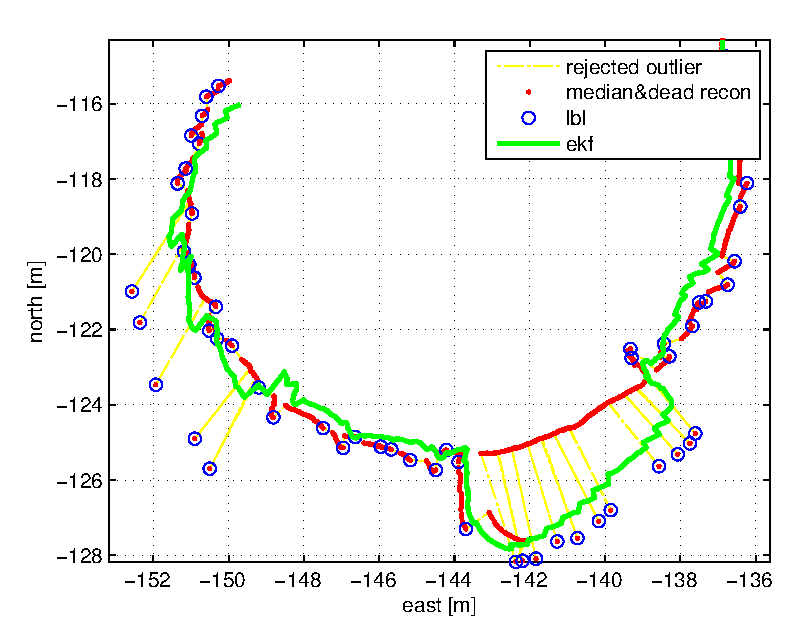
\includegraphics[width=0.5\linewidth]{results/fig/spiral-median-ekf.eps}} 
    %\subfigure[Spiral trajectory: LBL outliers filtered with EKF.] {\label{fig:spiral-ekf}
    %\includegraphics[width=0.45\linewidth]{results/fig/spiral-ekf.eps}}     
\end{figure}

\T{Square trajectories: } square trajectories were tested in low depths of a lake, with the GPS signal available to be used as a position reference and ground truth indication (Figures ~\ref{fig:no-gps}, ~\ref{fig:with-gps}). Dead reckoning navigation was used as a reference when controlling the vehicle movement during the experiment. This fact can cause slight confusion in analysis of the trajectory graphs since all the dynamics and forces were applied with respect to the dead reckoning navigation which is an estimated value, not the real existing one. It is a slightly inverse logic of testing, nevertheless further tests are yet to be accomplished. Emphasis of this experiment was to show that EKF can work successfully and analyse the main characteristics of the navigation design. It is likely that the GPS emulated square-shaped trajectories float as the elapsed path becomes longer. GPS signal available from the antenna located on the water surface is serving as a measure of absolute position within the lake - giving an idea about the actual vehicle position while it tries to moves within the boundaries of estimated dead reckoning position. 

Main issue when performing the square trajectory tests was significant imprecision of GPS signal. Many reasons can possibly influence the imprecision: from the weather conditions till surrounding objects. Basically anything that can affect the satellite visibility and the quality of the signal. Drifting can reach up to several meters which is unacceptable considering the trajectory length. Finally, the trajectory of the experiment itself is quite short ($ \approx 10 m $) to be seriously and accurately covered with precise GPS position update. Figure ~\ref{fig:gps} shows the tested trajectory and depicts the encountered amount of GPS imprecision.
\begin{figure}%[htb]
  \centering
    \subfigure[Coordinates of the tested square trajectory pasted on the lake map.] {\label{fig:gps-map}
	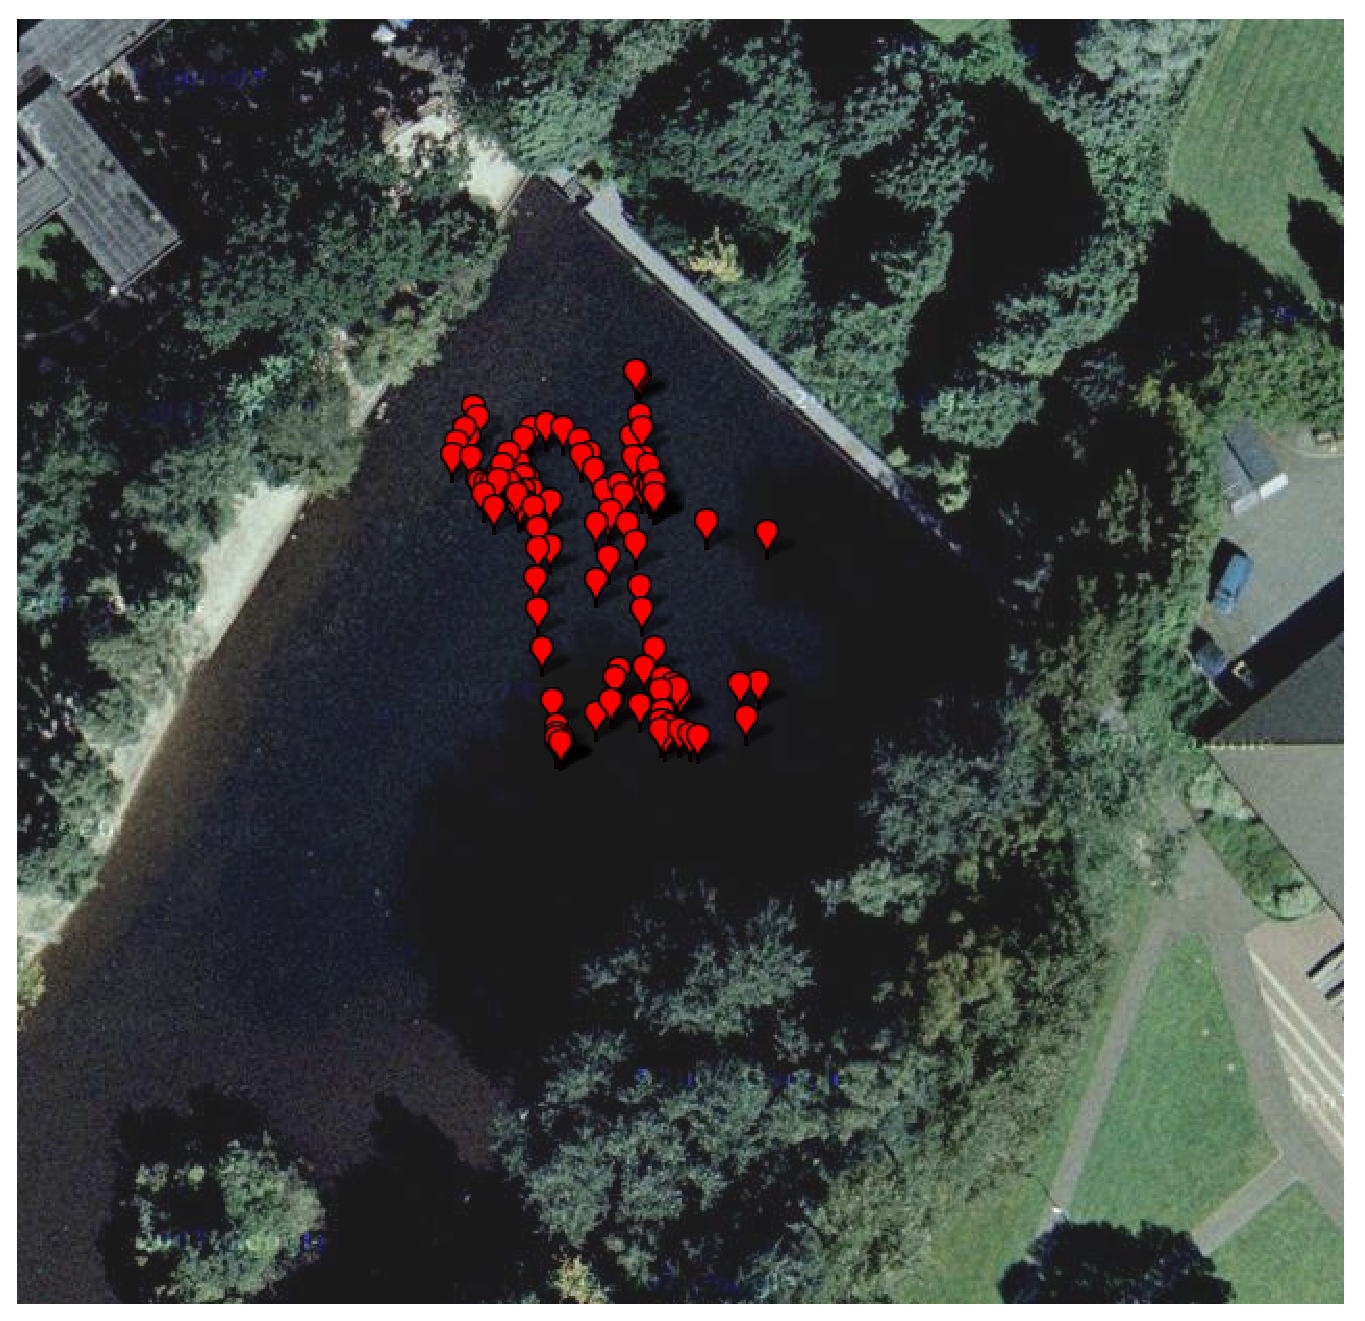
\includegraphics[width=0.48\linewidth]{results/fig/square-trajectory.eps}}
    \subfigure[GPS signal as it appears originally.] {\label{fig:gps-signal}
	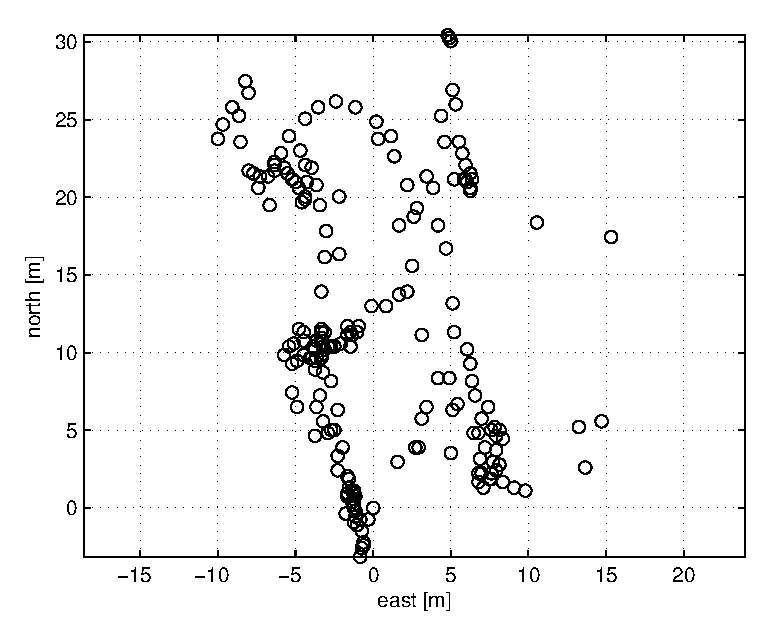
\includegraphics[width=0.48\linewidth]{results/fig/gps-signal.eps}}
\end{figure}

\T{Without GPS: } EKF localisation was tested in given conditions. Initially, only motion (inertial) sensors were used within the observations. That implies all the available linear and angular velocity sensors. Absolute position (raw GPS signal in this constellation) was not included in observations. EKF periodically updates (synchronous mode, \S~\ref{chap:methodology}), with the rate of 10 Hz. The aim was to measure the performance and the amount of drifting that occurs since the robot is intended to repeatedly attain square-like paths and return to the starting position in ideal scenario. It is useful to mention that proper parameter tuning can significantly change filtering performance. By giving more or less trust in particular measurement, or particular model behaviour, the role of certain parameters of dynamics (velocities, angular velocities) can be emphasized if necessary. Figure ~\ref{fig:no-gps} shows the performance of EKF without GPS position correction after one trajectory cycle, and the original path that was followed, recorded using GPS. Initial position was taken from the first GPS measurement and the first measurement can indeed be away from the real position due to GPS imprecision. Note that the control of the vehicle trajectory refers to dead-reckoning calculated north-east values, not some physical beacons with known position. At the time of reporting the experiments, testing were not fully completed with all the planned scenario variations. Localisation expectedly tends to perform with a significant drift without the absolute position update (Figure ~\ref{fig:square-1-noGps}). After the second square-shaped cycle (Figure ~\ref{fig:square-2-noGps}), EKF shows that it roughly tracks the shape of the trajectory, smooths it by filtering out the measurement outliers. Vehicle has returned approximately to the same position after each cycle. Drift gained when following one of the sides of the rectangular path was compensated with the same amount of drift but of the opposite sign that was active when taking the return direction. Enormous amount of drift is present since the information on absolute position is not considered. The first available GPS coordinate fixes the starting position and part of the initial position error is caused by being incapable of setting the initial position accurately.       
\begin{figure}%[htb]
  \centering
    \subfigure[N/E localisation.] {\label{fig:spiral2d}
	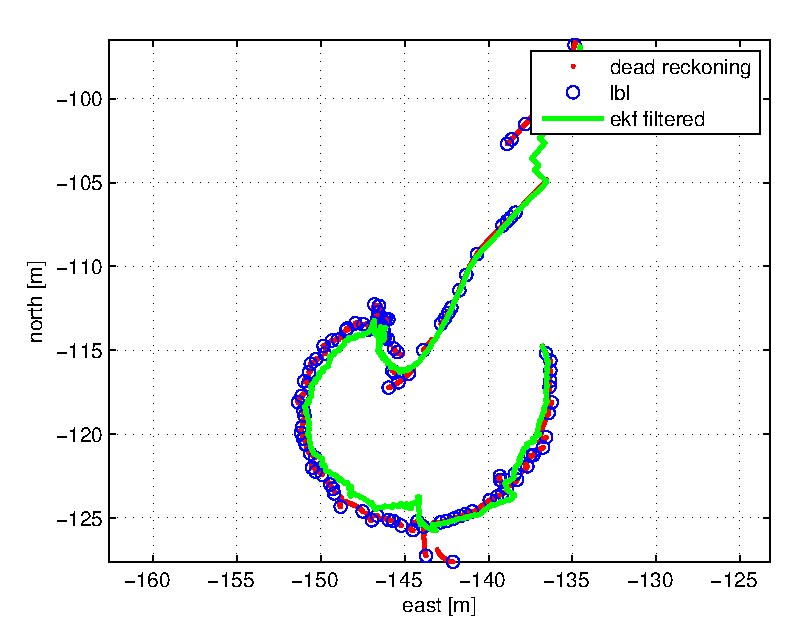
\includegraphics[width=0.48\linewidth]{results/fig/spiral2d.eps}}
    \subfigure[Depth.] {\label{fig:spiral-depth}
    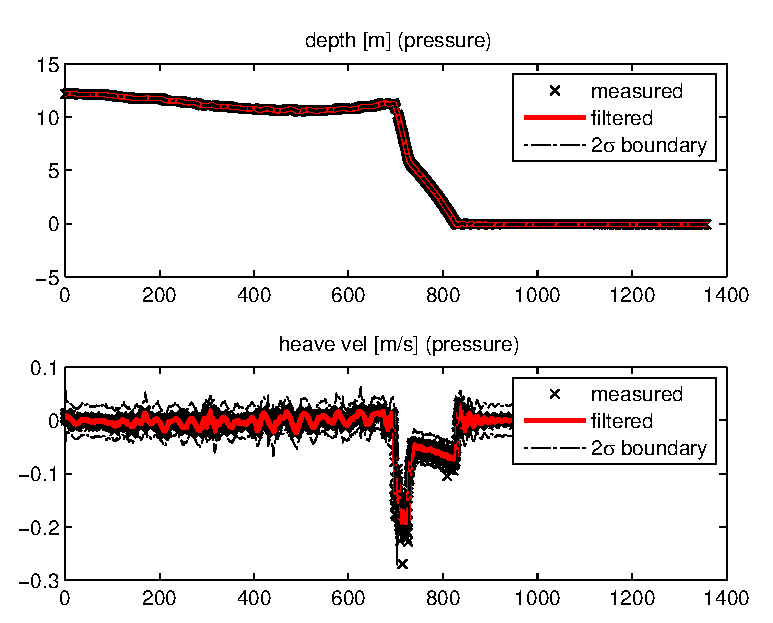
\includegraphics[width=0.48\linewidth]{results/fig/spiral-depth.eps}}
    % \\  
    %\subfigure[Path (temporary plot).] {\label{fig:spiral3d}
    %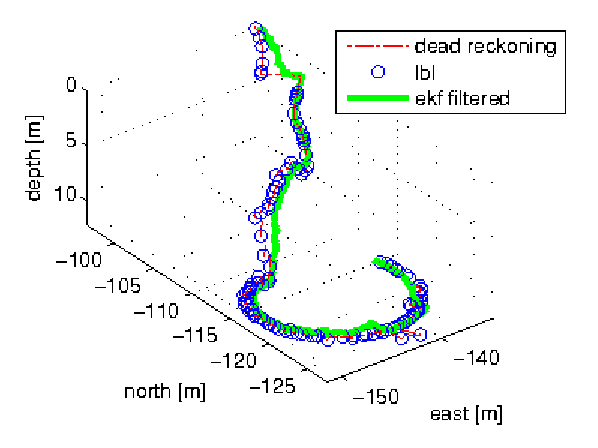
\includegraphics[width=0.8\linewidth]{results/fig/spiral3d.eps}} 
\end{figure}
\begin{figure}%[h]
  \centering
    \subfigure[EKF localisation after one cycle.] {\label{fig:square-1-noGps}
	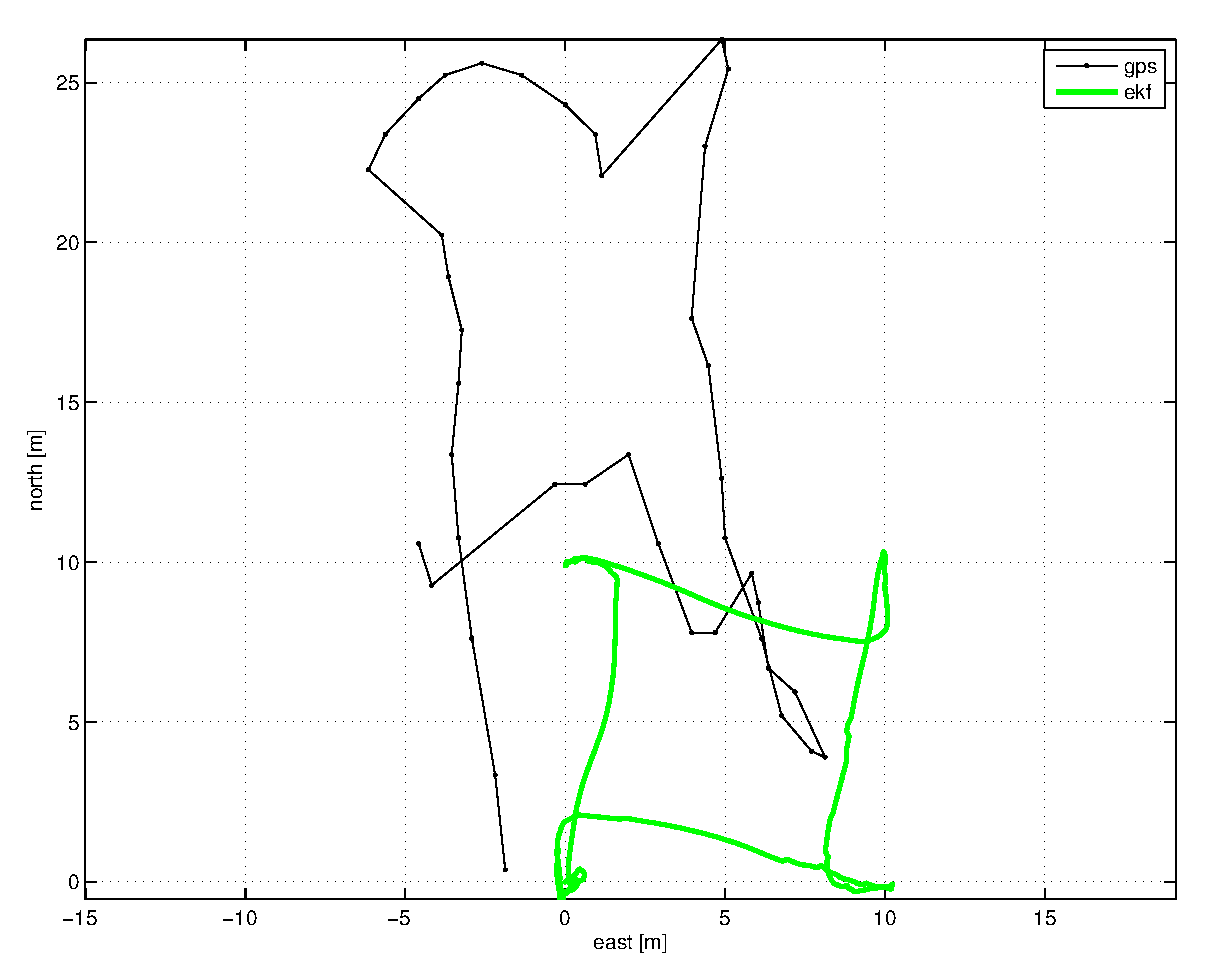
\includegraphics[width=0.48\linewidth]{results/fig/square1NoGps.eps}}
    \subfigure[EKF localisation after two cycles.] {\label{fig:square-2-noGps}
	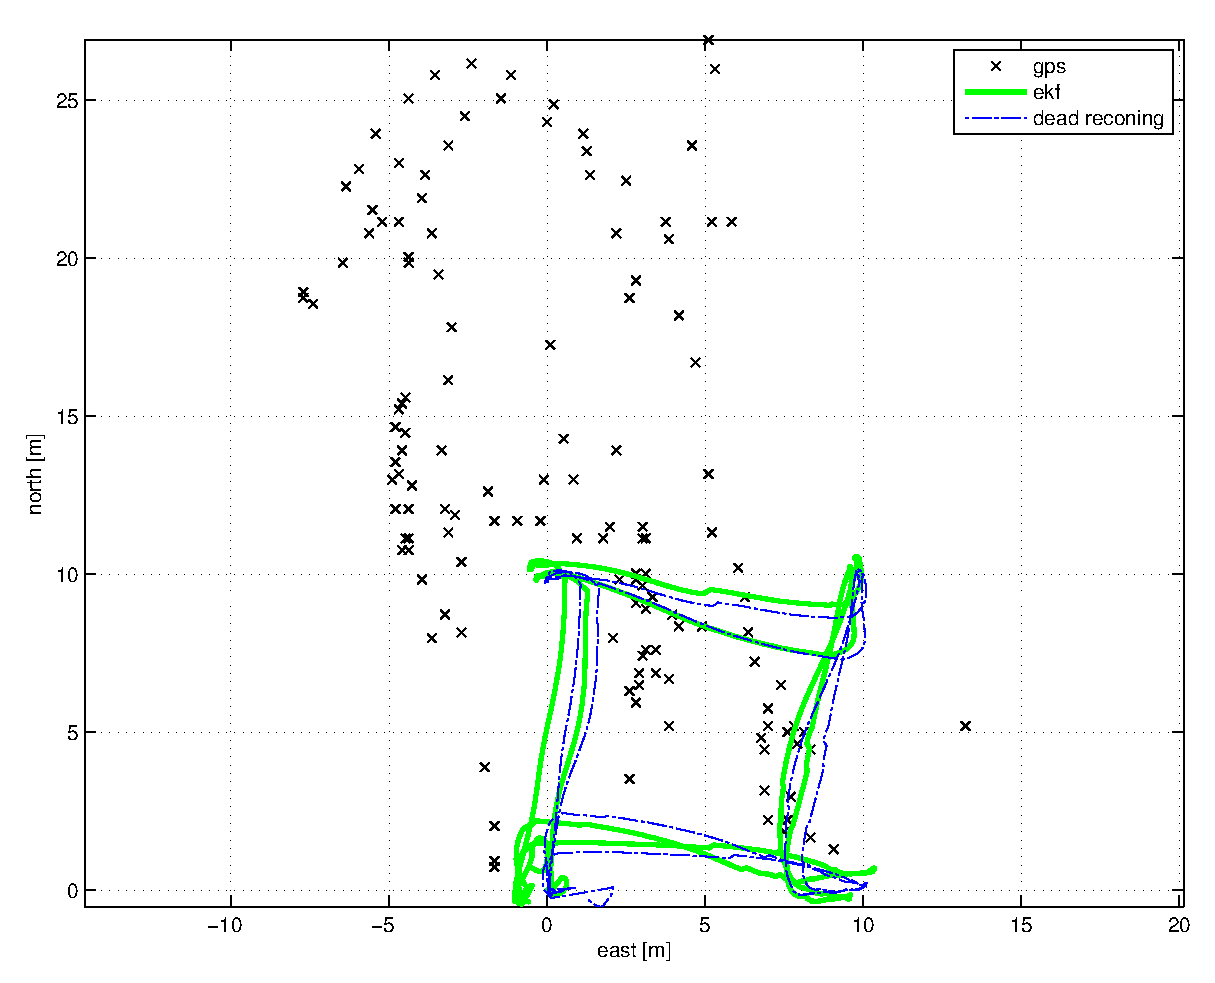
\includegraphics[width=0.48\linewidth]{results/fig/square2NoGps.eps}}\\
    %\subfigure[] {}
    %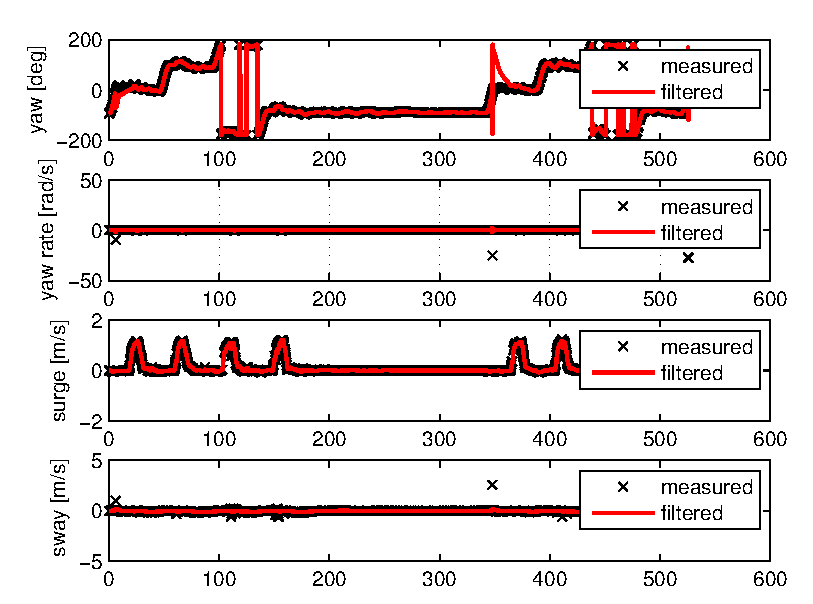
\includegraphics[width=0.6\linewidth]{results/fig/dynamics.eps}}
    \caption{EKF localisation using only inertial measurements as observation.}
    \label{fig:no-gps}
\end{figure}

\begin{figure}%[hb]%tb
  \centering
    \subfigure[Setting standard deviation of 1 m in uncertainty position observation (SDnorth = SDeast = 1.0 m).] {\label{fig:square-withGps-1}
	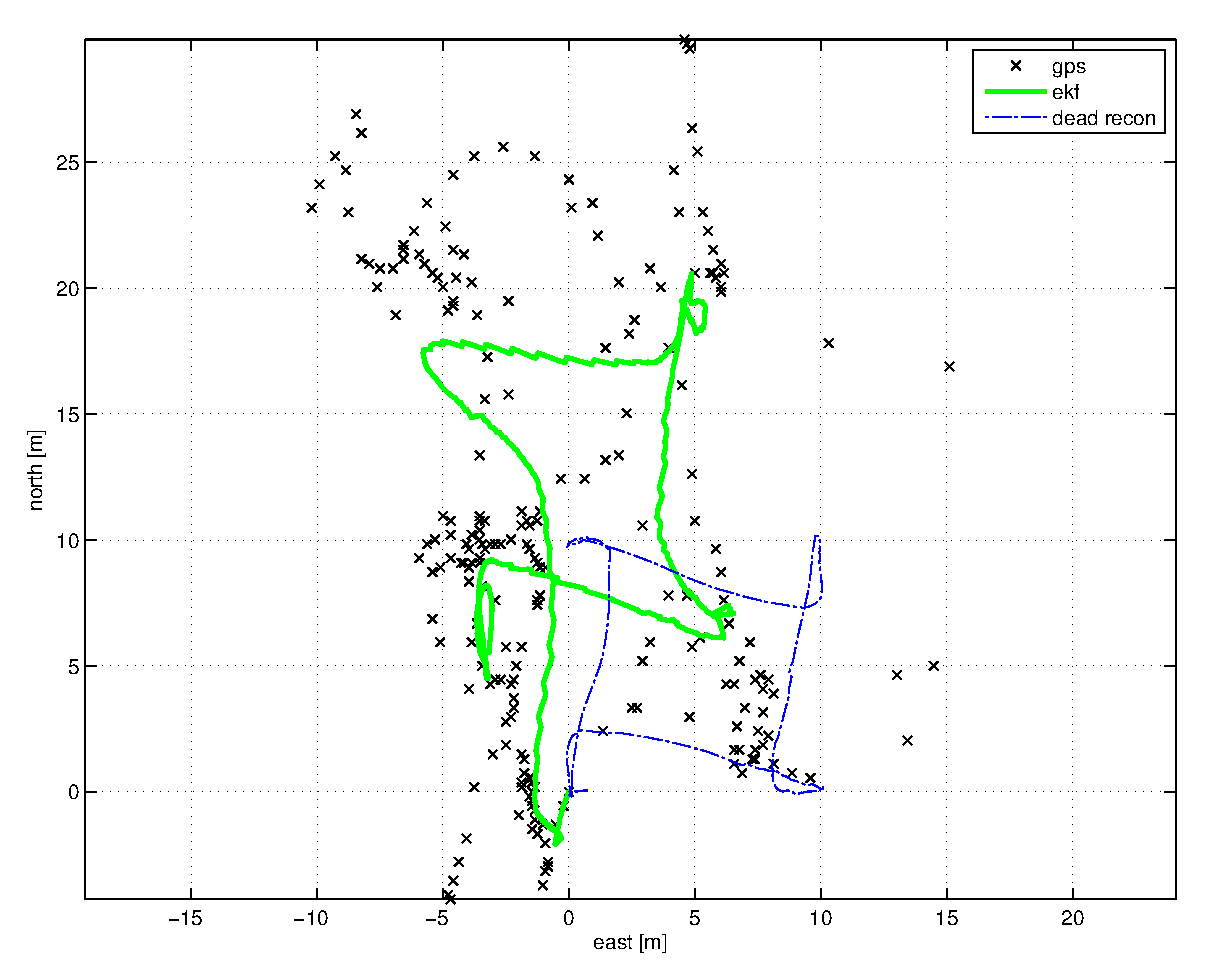
\includegraphics[width=0.48\linewidth]{results/fig/squareWithGps-10.eps}}
    \subfigure[EKF localisation after tuning the position uncertainty (SDnorth = SDeast = 0.5 m).] {\label{fig:square-withGps-2}
	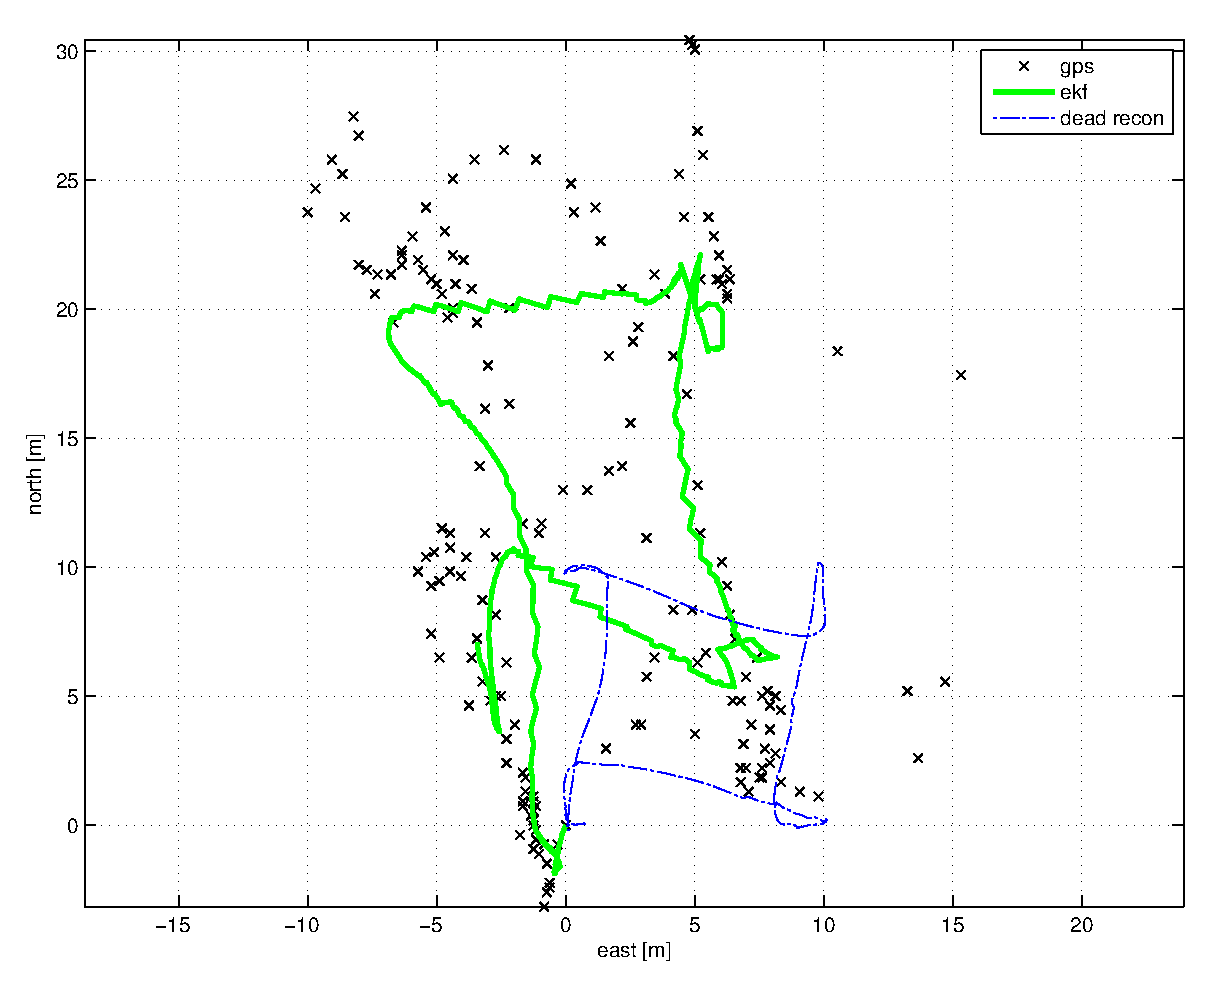
\includegraphics[width=0.48\linewidth]{results/fig/squareWithGps-05.eps}}
    %\\
    %\subfigure[Linear and angular velocities during square-shaped trajectory.] {\label{fig:square-dynamics}
    %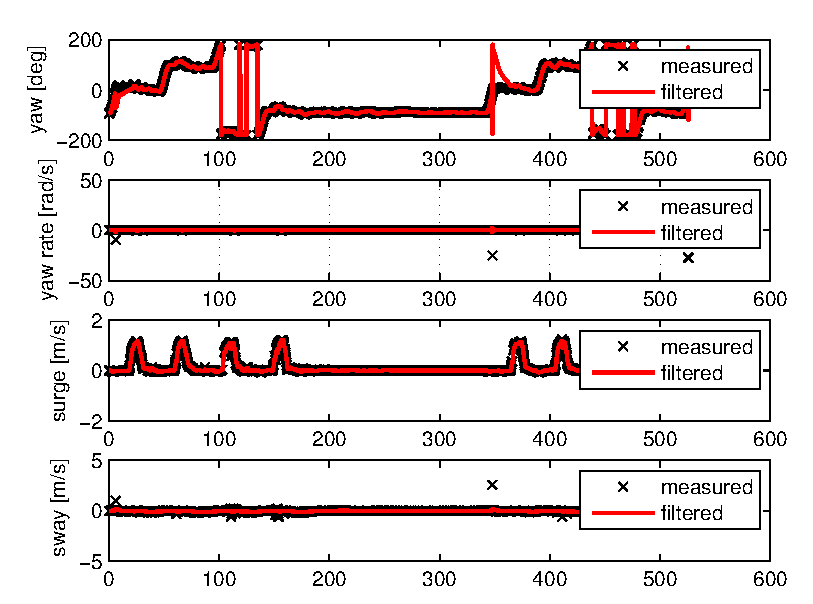
\includegraphics[width=0.45\linewidth]{results/fig/dynamics.eps}}
    \caption{EKF localisation aided with GPS position updates weighted by setting appropriate parameters.}
    \label{fig:with-gps}
\end{figure}
\begin{figure}
\centering
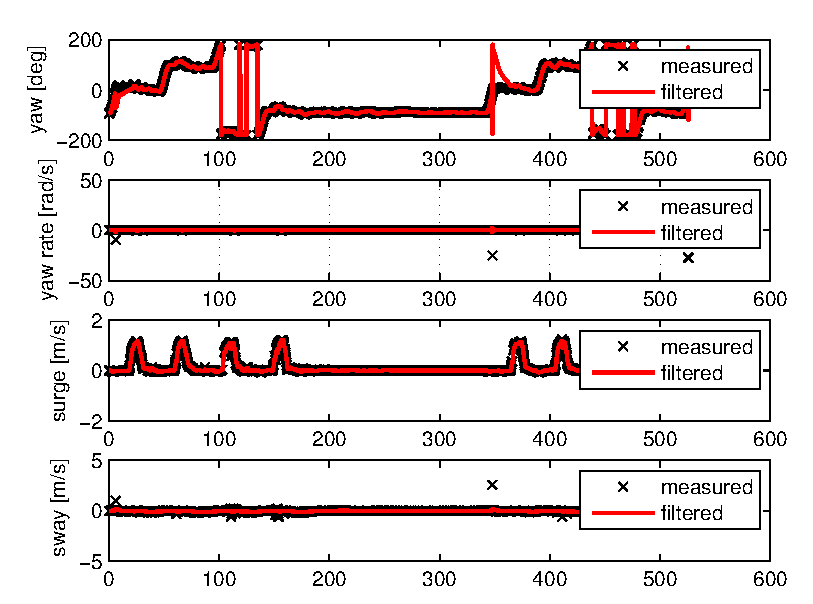
\includegraphics[width=0.6\linewidth]{results/fig/dynamics.eps}
\caption{Linear and angular velocities during square-shaped trajectory.}
\label{fig:square-dynamics}
\end{figure}
\T{With GPS: } Finally, GPS measurements were appended to the EKF observations. Localisation results were shown in Figure ~\ref{fig:with-gps} for two different level of confidence (variances) in position measurement. Naturally, giving extremely high confidence does not seem to be the best choice, however, some empirically deduced values in range of decimetres significantly correct the dead reckoning drift. Furthermore, EKF tends to filter the GPS measured north east coordinates, hence partially corrects the GPS imprecisions stated at the beginning. At this point it is evident why EKF is a great tool. Filter tries to satisfy the set uncertainty boundaries and fuse all the available information trying to make the most out of it combined together in one mathematical system. Moreover, fusing such imprecise and sketchy position data from GPS, still improves the localisation. Obtained trajectory tends to go towards what can be treated as expected path. From something that looked like a noisy collection of position observations at the beginning (Figure ~\ref{fig:gps-signal}), application of EKF together with sensor fusion enabled having generally better performance in navigation.     
%Combination of all relevant sensors gives in a Kalman filter state estimate results in more precise position and heading compared with instant (flat) usage of position and orientation measurements.  
%\subsection{Sensor selection}
%Design and performance test.
%\subsection{Using FOG for navigation improvement}
%How big is the improvement with respect to the distance travelled?

%%%%%%%%%%%%%%%%%%%%%%%%%%%%%%%%%%%%%%%%%%%%%%%%%%%%%%%%%%%%%%%%%%%%%%%%%%%%%%%%
\addtolength{\textheight}{-3cm}   % This command serves to balance the column lengths
                                  % on the last page of the document manually. It shortens
                                  % the textheight of the last page by a suitable amount.
                                  % This command does not take effect until the next page
                                  % so it should come on the page before the last. Make
                                  % sure that you do not shorten the textheight too much.

%%%%%%%%%%%%%%%%%%%%%%%%%%%%%%%%%%%%%%%%%%%%%%%%%%%%%%%%%%%%%%%%%%%%%%%%%%%%%%%%
\section{CONCLUSIONS AND FUTURE WORKS} \label{sec:concl}
\subsection{Conclusions}
The main focus of the work presented is practical application of Extended Kalman Filter for Ocean System Lab's Nessie AUV navigation module. EKF was designed to estimate the location of an underwater robot by processing real-time inertial and position information obtained from sensors. Furthermore, EKF algorithm was utilized as a framework for accomplishing sensor fusion - blending together measurements from different sensors as a part of the estimation process. The issues that were addressed in the thesis include suitable management of measurement tasks among mounted sensor devices and the role of EKF in correcting deficiencies. Specific case of heading measurement was tested, since this type of angular information is particularly important for the navigation. In conclusion, EKF proves to be useful navigation tool with several convenient features: capable of successfully combining together different sensory information into a location estimate that tends to be optimal with respect to set expectations, or recovering from the missing measurements, corrupted position information, outliers, or signal noise. Implementation of UKF for localisation would improve the accuracy of approximating nonlinearities in EKF at the same computational cost.
%satisfactory navigation performance and 
\subsection{Future Works}
Future work on improving localisation performance involves more trials with the vehicle trajectory fixed to known landmarks, so that the results of localisation could be thoroughly evaluated with trustful ground truth. Experiments that involve tilted vehicle movements could make an evaluation of the influence of the 5th DOF on the quality of localisation. EKF could be improved so that it works with control inputs - which could contribute in robustness of the localisation. Finally, the problem of correcting the absolute position with LBL information gives space for improvement since the measured position tends to be quite uncertain and prone to different sorts of noise. Solution for rejecting outliers could rely on some version of back-filtering - filtering based on history of received observations.
%%%%%%%%%%%%%%%%%%%%%%%%%%%%%%%%%%%%%%%%%%%%%%%%%%%%%%%%%%%%%%%%%%%%%%%%%%%%%%%%
\section{ACKNOWLEDGMENTS}
Author would like to thank VIBOT consortium and European Commission for sponsoring.  
%%%%%%%%%%%%%%%%%%%%%%%%%%%%%%%%%%%%%%%%%%%%%%%%%%%%%%%%%%%%%%%%%%%%%%%%%%%%%%%%
%%%%\begin{thebibliography}{99}
%%%%
%%%%\bibitem{c1}
%%%%J.G.F. Francis, The QR Transformation I, {\it Comput. J.}, vol. 4, 1961, pp 265-271.
%%%%
%%%%\bibitem{c2}
%%%%H. Kwakernaak and R. Sivan, {\it Modern Signals and Systems}, Prentice Hall, Englewood Cliffs, NJ; 1991.
%%%%
%%%%\bibitem{c3}
%%%%D. Boley and R. Maier, "A Parallel QR Algorithm for the Non-Symmetric Eigenvalue Algorithm", {\it in Third SIAM Conference on Applied Linear Algebra}, Madison, WI, 1988, pp. A20.
%\end{thebibliography}

\bibliographystyle{plain}
\bibliography{refs}
%\nocite{*}

\end{document}
